% Plantilla de documento para PFG usando memoriaPFC.cls

\documentclass{memoriaPFC}

%% ---------------------------------------------------
%% Datos del resumen y descriptores (para metadatos y resumen)
%% ---------------------------------------------------

\resumen{% 200-250 palabras
Este proyecto tiene como objetivo el diseño e implementación de un sistema inteligente integrado 
en una plataforma digital de comparación de precios de carburantes, desarrollada sobre Google 
Cloud Platform con una arquitectura de microservicios desplegada mediante Cloud Run y 
Cloud Functions. La solución, implementada con FastAPI en el backend y React en el frontend, 
permite a los usuarios consultar precios actualizados en tiempo real a partir de la API oficial 
del Ministerio para la Transición Ecológica, acceder a históricos de precios por estación 
de servicio y visualizar predicciones a siete días generadas mediante modelos de machine 
learning basados en LightGBM.
Más allá de la simple visualización de información, el sistema incorpora un módulo de 
recomendación de repostaje en ruta que, apoyándose en la API de Google Maps para el 
análisis geoespacial y la optimización de recorridos, determina qué estación resulta más 
conveniente económicamente para un trayecto definido por el usuario. Esta recomendación 
combina el precio actual, la evolución prevista y la desviación necesaria respecto al 
recorrido, evaluando el coste total del desplazamiento.
Los datos son gestionados mediante Neon Tech como almacén analítico principal y Cloud Storage 
para la persistencia de modelos y artefactos. La plataforma es accesible desde dispositivos 
móviles mediante una interfaz web responsive y contempla adicionalmente un asistente conversacional 
por voz construido sobre el protocolo MCP (Model Context Protocol), priorizando en todo momento la 
experiencia de usuario.
El proyecto integra competencias de ingeniería de software, análisis de datos e inteligencia 
artificial aplicada, constituyendo una solución tecnológica orientada al ahorro económico, 
la eficiencia energética y la toma de decisiones basada en datos.}

\descriptores{Proyecto, Ingeniería, Desarrollo, Documentación, Evaluación}


%% ---------------------------------------------------
%% Comienzo del documento
%% ---------------------------------------------------

\begin{document}

%% Selección de idioma del documento
\selectlanguage{spanish}  % Comentar esta línea para redactar en inglés

%% ----------------------
%% Materia preliminar
%% ----------------------

\frontmatter

%
\includepdf[pages=1]{../portada.pdf}          % Portada delantera (opcional)
%\includepdf[pages=1]{../portada_firmada.pdf}  % Portada firmada (opcional)

\resumenPersonalizado{
Este proyecto abordó el diseño e implementación de \textit{TankGo}, una plataforma
cloud-native de comparación de precios de carburantes y puntos de recarga eléctrica
en España, extendida con capacidades de inteligencia artificial y recomendación
geoespacial. El trabajo se enmarca en el área de la ingeniería del software y los
sistemas inteligentes, con aplicación directa de técnicas de análisis de datos,
aprendizaje automático y computación en la nube.

El desarrollo comprendió las siguientes fases: estudio del estado del arte y análisis
de soluciones existentes; planificación y definición de requisitos; diseño de la
arquitectura del sistema; implementación del backend con \textit{FastAPI} y base de
datos \textit{PostgreSQL} serverless sobre \textit{Neon Tech}; desarrollo del frontend
con \textit{React}; despliegue de la infraestructura en \textit{Google Cloud Platform}
mediante \textit{Cloud Run} y \textit{Cloud Functions}; e integración de un modelo
predictivo de precios basado en \textit{LightGBM} con horizonte de siete días.

El alcance específico del proyecto incluyó: la ingesta automatizada de datos desde la
API oficial del Ministerio para la Transición Ecológica, un módulo de recomendación
de repostaje en ruta apoyado en la API de Google Maps, una interfaz web
\textit{responsive} accesible desde dispositivos móviles, y un asistente conversacional
por voz construido sobre el protocolo MCP (\textit{Model Context Protocol}). El sistema
resultante constituye una solución funcional, escalable y orientada al ahorro
económico y la eficiencia energética en el transporte.
}{Computación en la nube, predicción de precios, aprendizaje automático, recomendación geoespacial, plataforma de carburantes.}

%% Índices
\tableofcontents
%\listoffigures        % Opcional
%\listoftables         % Opcional
%\lstlistoflistings    % Opcional (índice de código fuente)


%% ----------------------
%% Contenido principal
%% ----------------------

\mainmatter

\chapter*{Agradecimientos}
Deseo expresar mi agradecimiento a Diego López de Ipiña por el apoyo y la orientación prestados durante la realización de este Proyecto Fin de Grado. Asimismo, agradezco su labor en la asignatura en la que surgió la idea inicial de este trabajo, cuyo enfoque y desarrollo han sido fundamentales para la materialización del proyecto.

%% Contenido principal (usar \input para incluir capítulos externos)
\chapter{Capítulo Primero - Introducción }
La presente memoria recoge el trabajo realizado en el marco del Proyecto de Fin de Grado del Grado en Ingeniería Informática. Este proyecto integra de forma aplicada los conocimientos y competencias adquiridas a lo largo de la titulación, especialmente en las áreas de ingeniería del software, arquitecturas en la nube, gestión y procesamiento de datos, sistemas inteligentes y análisis predictivo.

El proyecto desarrollado consiste en la evolución del prototipo académico \textit{TankGo} \cite{Alvis2025TankGo} hacia una plataforma software completa orientada a la consulta, comparación y análisis de precios de combustibles y puntos de recarga eléctrica. La solución propuesta se concibe como un sistema integrado desplegado en entorno cloud que combina distintos componentes tecnológicos: ingestión y persistencia de datos, procesamiento distribuido, modelos de predicción basados en aprendizaje automático, algoritmos de recomendación geoespacial y un sistema de asistencia conversacional para la interacción con el usuario.

Este proyecto se enmarca en el área de Sistemas de Información e Ingeniería del Software, al abordar el diseño, desarrollo, despliegue y evaluación de una solución tecnológica orientada a resolver un problema real mediante una arquitectura escalable y modular.

\section{Motivación}
El sector de las gasolineras y los puntos de recarga eléctrica presenta una alta variabilidad en precios y disponibilidad, lo que genera incertidumbre en los usuarios y dificulta la toma de decisiones. Aunque existen herramientas que permiten consultar precios actuales, pocas soluciones integran funcionalidades avanzadas como predicción a corto plazo, recomendación basada en rutas o análisis geoespacial optimizado dentro de una misma plataforma.

La motivación principal de este proyecto es explorar la viabilidad técnica de integrar en un único sistema distintos enfoques tecnológicos tales como analítica de datos, predicción, recomendación y asistencia inteligente con el fin de aportar un valor respecto a soluciones convencionales.

El proyecto es una evolución de un desarrollo académico previo, ampliando su alcance, mejorando la arquitectura y profundizando en la fundamentación técnica y metodológica exigida en un Proyecto Fin de Grado.

\section{Estructura de la memoria}
La memoria se ha estructurado en capítulos que recogen de manera ordenada los distintos aspectos del proyecto. Tras esta introducción, se presentan los antecedentes y la justificación técnica del sistema, incluyendo el estado del arte y el análisis de soluciones existentes.

Posteriormente, se definen los objetivos y el alcance del proyecto, seguidos de la planificación temporal y de recursos, el presupuesto estimado y la metodología adoptada.

El núcleo del documento lo constituye el capítulo de desarrollo, donde se detallan la especificación de requisitos, el diseño del sistema, las decisiones tecnológicas adoptadas, la implementación y el plan de pruebas. Finalmente, se incluye una valoración ética del proyecto, las conclusiones obtenidas y posibles líneas futuras de mejora, junto con la bibliografía y los anexos correspondientes.
% !TEX root = ../main.tex
\chapter{Capítulo Segundo - Antecedentes y Justificación  }
\section{Situación actual del sector de gasolineras}
En los últimos años el sector energético vinculado a la movilidad ha experimentado una transformación impulsada por factores económicos, regulatorios y medioambientales. La volatilidad del precio de los combustibles fósiles, el aumento progresivo del parque de vehículos eléctricos y las políticas de transición energética han incrementado la necesidad de información precisa para la toma de decisiones de repostaje y recarga \cite{expansion_motor_2026_01_12}.

La coexistencia de distintas fuentes energéticas (gasolina, diésel, GLP, electricidad) introduce mayor complejidad en el proceso de decisión del usuario. Además, los precios presentan variaciones relevantes entre estaciones de servicio cercanas e incluso fluctuaciones temporales a corto plazo.

Desde las administraciones públicas se ha promovido la publicación de datos abiertos sobre precios de carburantes y localización de puntos de recarga\cite{datosgob_carburantes,geoportal_gasolineras}, lo que ha facilitado el desarrollo de herramientas digitales de consulta.

\section{Problemas detectados}

Tras un análisis del estado actual de las soluciones tecnológicas en el sector de la movilidad, se han identificado las siguientes deficiencias técnicas y funcionales que motivan el desarrollo de este proyecto:

\begin{itemize}
    \item \textbf{Heterogeneidad y dispersión de datos:} La información de precios y puntos de carga reside en silos aislados (OpenData gubernamental, APIs privadas, \textit{scrapers}), lo que dificulta una visión unificada y coherente en tiempo real.
    \item \textbf{Carácter estático de la consulta:} Las plataformas actuales funcionan como visores de datos puntuales, careciendo de un análisis histórico que permita comprender las fluctuaciones del mercado.
    \item \textbf{Ausencia de capacidad predictiva:} No se integran modelos de inteligencia artificial que asistan al usuario en la toma de decisiones anticipadas (¿conviene repostar hoy o esperar a mañana?).
    \item \textbf{Desconexión con la planificación geoespacial:} La búsqueda de estaciones suele ser radial o por cercanía, ignorando la optimización del coste energético total en función de una ruta planificada.
    \item \textbf{Brecha digital entre energías:} Existe una fragmentación tecnológica entre los sistemas de gestión de combustibles tradicionales y la infraestructura de movilidad eléctrica (EV), impidiendo una gestión híbrida eficiente.
    \item \textbf{Falta de asistencia inteligente:} La interacción usuario-sistema sigue patrones rígidos de formularios, desaprovechando las capacidades actuales de los sistemas conversacionales y el procesamiento de lenguaje natural (NLP).
\end{itemize}

Estos problemas representan una oportunidad para diseñar una arquitectura que no solo centralice la información, sino que aplique capas de inteligencia de datos para transformar la información bruta en conocimiento accionable.

\section{Estado del arte}

El estudio del estado del arte en este trabajo abarca tres ámbitos tecnológicos diferenciados que convergen en la solución propuesta: la predicción de precios energéticos mediante aprendizaje automático, los sistemas de recomendación geoespacial aplicados a la movilidad y las arquitecturas cloud orientadas al procesamiento de datos en tiempo real.

\subsection{Predicción de precios de combustibles}

La predicción de precios en mercados energéticos es un problema ampliamente estudiado en la literatura. Los enfoques clásicos basados en modelos estadísticos como ARIMA o GARCH han sido gradualmente desplazados por técnicas de aprendizaje automático que capturan relaciones no lineales y dependencias temporales complejas.

En el contexto de los carburantes, estudios recientes demuestran que los modelos de \textit{gradient boosting} (en particular LightGBM) ofrecen un rendimiento superior en tareas de regresión sobre series temporales de precios al incorporar variables exógenas como el precio del crudo Brent, la estacionalidad o indicadores macroeconómicos \cite{LAHMIRI2024105008}. Lahmiri y Bekiros destacan que la incorporación de datos de mercados financieros como covariables mejora significativamente la capacidad predictiva de estos modelos frente a enfoques univariantes.

Paralelamente, la literatura señala la utilidad de los modelos de regresión cuantílica para estimar no solo el valor esperado del precio futuro, sino intervalos de confianza que permiten una toma de decisiones más informada \cite{s24124013}. Este enfoque resulta especialmente relevante en el contexto de la presente plataforma, donde la incertidumbre del precio es tan relevante como la predicción puntual.

Los enfoques de \textit{Deep Learning}, como las redes LSTM (\textit{Long Short-Term Memory}), han mostrado capacidad para modelar dependencias temporales a largo plazo. Sin embargo, su coste computacional y menor interpretabilidad los posicionan como alternativas a evaluar de forma comparativa frente a los modelos de \textit{gradient boosting}, cuya eficiencia en datos tabulares y series temporales cortas está ampliamente documentada \cite{LAHMIRI2024105008}.

\subsection{Sistemas de recomendación en movilidad}

Los sistemas de recomendación aplicados a la movilidad han evolucionado desde soluciones basadas en proximidad geográfica (\textit{nearest neighbor}) hacia enfoques que integran múltiples criterios: coste, disponibilidad, tiempo de desvío y preferencias del usuario. En el ámbito de los puntos de recarga eléctrica, la literatura recoge modelos de optimización multicriterio que consideran la autonomía del vehículo, la disponibilidad de conectores y el coste de la energía \cite{mitma_esmovilidad}.

En el contexto de gasolineras, la recomendación basada en rutas (a diferencia de la búsqueda por cercanía) implica la definición de un corredor geométrico alrededor del trayecto planificado y la evaluación de estaciones dentro de dicho corredor según una función de puntuación ponderada. Este enfoque, adoptado en la presente plataforma, minimiza el desvío total mientras optimiza el coste energético del trayecto.

La integración de servicios de enrutamiento como OpenRouteService (ORS) u OSRM como backends intercambiables es una práctica consolidada en el desarrollo de aplicaciones de movilidad de código abierto, permitiendo flexibilidad entre precisión y coste operativo.

\subsection{Arquitecturas cloud para datos en tiempo real}

Las arquitecturas de microservicios desplegadas en entornos \textit{cloud-native} se han consolidado como el paradigma dominante para el desarrollo de plataformas de datos a escala. Frente a las arquitecturas monolíticas tradicionales, el modelo de microservicios ofrece desacoplamiento funcional, escalabilidad independiente por componente y resiliencia ante fallos parciales \cite{Gartner2026Trends}.

En el ámbito de la ingesta de datos abiertos gubernamentales, la federación de fuentes heterogéneas (APIs REST, portales de datos abiertos, servicios de terceros) requiere capas de normalización y persistencia que garanticen la coherencia del dato. La adopción de formatos columnar como Apache Parquet para la exportación de datos históricos y su almacenamiento en servicios de objeto (\textit{blob storage}) como Google Cloud Storage es una práctica ampliamente adoptada en pipelines de \textit{machine learning} que requieren reproducibilidad y versionado del dato \cite{s24124013}.

El despliegue serverless mediante contenedores en plataformas como Google Cloud Run representa una tendencia creciente que reduce la carga operativa de gestión de infraestructura, permitiendo al equipo de desarrollo centrarse en la lógica de negocio. Esta aproximación se alinea con los patrones de arquitectura adaptativa que Gartner identifica como prioritarios para el ciclo 2025-2026 \cite{Gartner2026Trends}.

\subsection{Asistentes conversacionales en aplicaciones de dominio específico}

El uso de modelos de lenguaje de gran escala (LLM) como componente de interfaces conversacionales en aplicaciones de dominio específico ha experimentado una adopción acelerada. La integración mediante protocolos estandarizados como el \textit{Model Context Protocol} (MCP) permite exponer capacidades del sistema backend como herramientas (\textit{tools}) invocables por el modelo, habilitando una capa de razonamiento sobre datos en tiempo real sin comprometer la arquitectura subyacente.

En el contexto de la movilidad, los asistentes de voz con capacidad de \textit{tool calling} representan una evolución respecto a los chatbots basados en flujos predefinidos, al poder responder a consultas abiertas del tipo \enquote{¿cuál es la gasolinera más barata en mi ruta a Bilbao?} mediante la composición dinámica de llamadas a la API del sistema.


\section{Soluciones existentes y limitaciones}

El mercado actual de aplicaciones para la consulta de precios de combustibles y puntos de recarga eléctrica en España ofrece diversas soluciones tanto de carácter oficial como de terceros. Su análisis permite identificar el espacio de mejora que justifica la propuesta de este proyecto.

\subsection{Plataformas gubernamentales}

El Ministerio para la Transición Ecológica y el Reto Demográfico (MITECO) mantiene el 
\textit{Geoportal de la Energía} \cite{geoportal_gasolineras}, que ofrece una interfaz de 
consulta de precios de carburantes en tiempo real basada en los datos del Ministerio de Industria. 
Si bien constituye la fuente de referencia oficial y su API REST es de acceso público 
\cite{datosgob_carburantes}, la interfaz de usuario presenta limitaciones notables: 
no dispone de funcionalidad de comparación histórica, no integra información de puntos 
de recarga eléctrica y carece de cualquier capacidad predictiva o de recomendación, asi como la falta de una experiencia de
usuario moderna e interactiva. La plataforma se limita a mostrar datos puntuales sin ofrecer herramientas de análisis o soporte a la decisión, lo que reduce su utilidad para el usuario final.

De forma análoga, la plataforma \textit{es-Movilidad} del MITECO \cite{mitma_esmovilidad} agrega información sobre infraestructura de recarga eléctrica, pero opera como un sistema independiente y no integrado con la información de combustibles convencionales, reproduciendo la fragmentación ya señalada en el análisis de problemas.

\subsection{Aplicaciones de terceros}

Existen aplicaciones móviles ampliamente utilizadas como \textit{Gasolineras España}, \textit{Waze} (con integración parcial de precios) o \textit{GasBuddy} en otros mercados, que abordan parcialmente el problema de la búsqueda por proximidad. No obstante, estas soluciones presentan limitaciones estructurales comunes:

\begin{itemize}
    \item \textbf{Ausencia de predicción:} Ninguna de las soluciones identificadas incorpora modelos de predicción de precios a corto plazo que orienten la decisión temporal de repostaje.
    \item \textbf{Recomendación por ruta limitada:} La optimización basada en trayectos planificados (corredor de ruta con función de coste ponderado) no está presente en las soluciones de referencia analizadas.
    \item \textbf{Fragmentación entre energías:} La gestión conjunta de combustibles convencionales y puntos de recarga eléctrica en una única interfaz unificada es inexistente en las soluciones actuales del mercado español.
    \item \textbf{Falta de interacción conversacional:} La interacción mediante lenguaje natural para consultas complejas no está disponible en ninguna de las plataformas analizadas.
    \item \textbf{Dependencia de datos crowdsourced:} Algunas plataformas dependen de aportaciones de usuarios para actualizar precios, introduciendo latencia y potencial sesgo en la información.
\end{itemize}

\subsection{Síntesis comparativa}

La Tabla~\ref{tab:comparativa_soluciones} resume de forma esquemática las capacidades de las principales soluciones existentes frente a las funcionalidades que incorpora el sistema propuesto.

\begin{table}[h]
\centering
\caption{Comparativa de funcionalidades entre soluciones existentes y TankGo}
\label{tab:comparativa_soluciones}
\begin{tabular}{lcccc}
\hline
\textbf{Funcionalidad} & \textbf{Geoportal} & \textbf{Apps móviles} & \textbf{es-Movilidad} & \textbf{TankGo (PFG)} \\
\hline
Precios en tiempo real     & \checkmark & \checkmark & --         & \checkmark \\
Historial de precios       & --         & Parcial    & --         & \checkmark \\
Predicción de precios      & --         & --         & --         & \checkmark \\
Recomendación por ruta     & --         & Parcial    & --         & \checkmark \\
Integración EV             & --         & --         & \checkmark & \checkmark \\
Asistente conversacional   & --         & --         & --         & \checkmark \\
API pública documentada    & \checkmark & --         & --         & \checkmark \\
Arquitectura cloud-native  & --         & --         & --         & \checkmark \\
\hline
\end{tabular}
\end{table}

Esta síntesis pone de manifiesto que, si bien existen soluciones parciales para cada funcionalidad de forma aislada, ninguna plataforma del mercado español integra el conjunto de capacidades propuesto en este trabajo. La propuesta de valor de TankGo reside precisamente en esa integración, que trasciende la suma de las partes para ofrecer un sistema de soporte a la decisión coherente y orientado al usuario.


\section{Origen del proyecto y evolución}
El presente proyecto parte de un prototipo académico desarrollado por el autor en la asignatura \textit{Desarrollo Avanzado de Aplicaciones para la Web de Datos} \cite{Alvis2025TankGo}. Dicho sistema inicial, denominado \textit{TankGo}, permitía la consulta de precios de estaciones de servicio mediante la federación de fuentes de datos abiertos y una visualización geoespacial básica. No obstante, aquel desarrollo presentaba una arquitectura acotada a objetivos formativos.
El actual Trabajo de Fin de Grado retoma esa base tecnológica para transformarla en una plataforma robusta y profesional. Esta evolución no es meramente incremental, sino que supone una redefinición del sistema bajo tres ejes estratégicos alineados con tendencias recientes de la industria del \textit{software}, especialmente en adopción de IA y arquitecturas de plataforma escalables en entornos \textit{cloud} \cite{Gartner2026Trends}.

\begin{enumerate}
    \item \textbf{Infraestructura y persistencia escalable:} Se migra hacia una arquitectura \textit{cloud-native} capaz de procesar datos masivos. Esto permite la ingesta de flujos de datos en tiempo real, una capacidad crítica para mitigar riesgos en el sector energético \cite{s24124013}.
    \item \textbf{Inteligencia de datos y modelado predictivo:} Se incorpora un motor de pronóstico de precios. A diferencia del prototipo original, se plantea una evaluación comparativa de distintos modelos (p. ej., LightGBM, XGBoost y enfoques de \textit{Deep Learning}) para seleccionar la alternativa con mejor equilibrio entre precisión, coste computacional e interpretabilidad en el contexto del proyecto \cite{LAHMIRI2024105008,s24124013}.
\end{enumerate}

Con este enfoque, el sistema evoluciona de una herramienta informativa hacia un sistema de apoyo a la decisión, alineado con las exigencias de un sistema de información avanzado.

\section{Justificación técnica y académica}

Desde el punto de vista \textbf{técnico}, el proyecto trasciende la implementación de software para convertirse en un ejercicio de integración de múltiples disciplinas de la Ingeniería Informática. La solución se fundamenta en la convergencia de:
\begin{itemize}
    \item \textbf{Arquitectura de Sistemas:} Diseño de una infraestructura modular \textit{cloud-native} que garantiza escalabilidad y disponibilidad.
    \item \textbf{Gestión de Datos y Analítica:} Implementación de flujos de ingesta y persistencia políglota para el tratamiento de series temporales de precios.
    \item \textbf{Inteligencia Computacional:} Incorporación de modelos predictivos que, como sugiere la literatura reciente \cite{LAHMIRI2024105008}, son esenciales para transformar datos brutos en conocimiento accionable en el sector energético.
    \item \textbf{Ingeniería de Interfaces:} Desarrollo de sistemas de interacción avanzada, incluyendo asistencia conversacional y visualización geoespacial compleja.
\end{itemize}

Desde la \textbf{perspectiva académica}, este trabajo se justifica como una síntesis integral de las competencias del Grado en Ingeniería Informática. El proyecto no solo valida la capacidad técnica del autor, sino su madurez metodológica al:
\begin{itemize}
    \item \textbf{Sintetizar conocimientos:} Unificar áreas como la Inteligencia Artificial, el Desarrollo Web y la Gestión de Proyectos en un único ecosistema coherente.
    \item \textbf{Rigor investigativo:} Fundamentar las decisiones de diseño en un análisis del estado del arte y tendencias tecnológicas globales para 2026 \cite{Gartner2026Trends}.
    \item \textbf{Gestión de Ingeniería:} Aplicar una planificación formal, estimación de costes operativos (OpEx) y una evaluación técnica basada en métricas de rendimiento y calidad de software.
    \item \textbf{Pensamiento crítico:} Evaluar de forma objetiva las limitaciones del sistema y proponer líneas de evolución futura dentro de la ética profesional y la sostenibilidad.
\end{itemize}

\subsection{Alineación con los Objetivos de Desarrollo Sostenible (ODS)}

La Agenda 2030 de las Naciones Unidas establece una hoja de ruta global hacia la sostenibilidad a través de 17 objetivos \cite{onu_ods_goals}. Aunque el presente trabajo es de naturaleza técnica y computacional, su despliegue en el sector de la movilidad inteligente (\textit{Smart Mobility}) permite una alineación estratégica con las siguientes metas:

\begin{itemize}
    \item \textbf{ODS 7 (Energía asequible y no contaminante):} El sistema contribuye a la meta 7.3 (eficiencia energética) mediante la democratización y transparencia de datos. Al integrar en una única interfaz precios de combustibles y puntos de recarga eléctrica, se facilita la transición hacia modelos de movilidad más sostenibles y económicamente eficientes.
    \item \textbf{ODS 9 (Industria, innovación e infraestructura):} Esta es la vinculación más directa del proyecto. La transformación de fuentes de datos heterogéneas en un Sistema de Soporte a la Decisión (DSS) mediante \textit{cloud computing} e Inteligencia Artificial promueve el desarrollo de infraestructuras digitales resilientes e innovadoras \cite{mitma_esmovilidad}. Se fomenta el uso de tecnologías abiertas y estándares de interoperabilidad, pilares de la industria 4.0.
    \item \textbf{ODS 12 (Producción y consumo responsables):} La plataforma empodera al usuario final con herramientas de analítica predictiva \cite{LAHMIRI2024105008}, permitiendo un consumo más racional. La optimización de rutas basada en el coste energético reduce el desperdicio de recursos y fomenta una planificación logística más consciente.
    \item \textbf{ODS 13 (Acción por el clima):} Al facilitar la localización y gestión de puntos de recarga eléctrica frente a los combustibles fósiles, el proyecto actúa como un catalizador tecnológico para la reducción de emisiones de CO2 en el transporte por carretera, alineándose con las estrategias europeas de descarbonización.
\end{itemize}

Es importante destacar que, si bien el impacto directo es modesto debido al carácter académico del proyecto, la arquitectura propuesta demuestra cómo la digitalización y el procesamiento inteligente de datos son habilitadores críticos para alcanzar las metas de sostenibilidad nacional e internacional \cite{gob_agenda2030_espana}.

% !TEX root = ../main.tex
% =========================================================
%  CAPÍTULO 3 — MARCO TECNOLÓGICO
% =========================================================
 
\chapter{Capítulo tercero - Marco tecnológico}
 
La elección de las tecnologías que dan soporte a TankGo no ha sido arbitraria sino que responde
a un análisis previo de alternativas en el que se han ponderado criterios de
rendimiento, madurez del ecosistema, compatibilidad con el modelo de despliegue
cloud-native, coste operativo y alineación con las competencias adquiridas durante el
grado. Este capítulo documenta dicho análisis y justifica las decisiones adoptadas,
organizando las tecnologías según la capa arquitectónica en la que operan.
 
% ---------------------------------------------------------
\section{Capa de presentación: React y Leaflet.js}
% ---------------------------------------------------------
 
\subsection{React como framework de interfaz de usuario}
 
El cliente web de TankGo está desarrollado con \textbf{React 19}\cite{react}, la biblioteca de
interfaz de usuario de Meta. React adopta un paradigma declarativo basado en
componentes reutilizables y un DOM virtual que minimiza las operaciones de
renderizado sobre el árbol real, lo que resulta crítico en una aplicación como
TankGo, donde el mapa puede contener miles de marcadores que se actualizan
dinámicamente en función del viewport.
 
Entre las alternativas evaluadas se consideraron Vue.js y Angular \cite{vuejs,angular}. Angular, aunque
ofrece un entorno completo con \textit{dependency injection} integrada, introduce
una curva de aprendizaje significativa y un tamaño de bundle elevado para un
proyecto de alcance académico. Vue.js es una opción intermedia válida, pero su
ecosistema de integración con librerías cartográficas como Leaflet es menos maduro
que el de React, donde \texttt{react-leaflet}\cite{react_leaflet} ofrece una capa de abstracción directa sobre los componentes de ciclo de vida.
La prevalencia de React en el mercado laboral, alcanzando el 44,7\,\% según la encuesta anual de Stack Overflow de 2025, así 
como la familiaridad del autor con
la biblioteca, motivaron la elección final \cite{stackoverflow_survey_2025}.
 
\subsection{Leaflet.js como motor cartográfico}
 
La visualización geoespacial es clave en la experiencia de usuario de TankGo.
Para renderizar el mapa interactivo se evaluaron tres opciones principales: la API
de Google Maps, Mapbox GL JS y Leaflet.js.
 
La API de Google Maps queda descartada por su modelo de precios, que penaliza el
uso intensivo de marcadores y limita la personalización de las capas de datos sin
incurrir en costes adicionales \cite{logrocket_leaflet_guide}. Mapbox GL JS, si bien
ofrece renderizado WebGL de alto rendimiento y estilos vectoriales personalizables,
cambió su licencia de código abierto BSD a una licencia propietaria a partir de la
versión 2 en 2020, lo que excluye su uso libre en proyectos sin garantía de
continuidad de acceso \cite{geoapify_map_comparison}.
 
Leaflet.js es una biblioteca de código abierto bajo licencia BSD-2, pesa
aproximadamente 42\,KB en su versión minificada y ofrece un ecosistema de
\textit{plugins} especialmente extenso \cite{logrocket_leaflet_guide}. Su
integración nativa con teselas de OpenStreetMap elimina dependencias de
terceros propietarios, garantizando la continuidad del servicio sin costes de
API. El plugin \texttt{react-leaflet} \cite{react_leaflet} permite declarar capas y marcadores como
componentes React, integrándose de forma natural con el modelo de estado de la
aplicación. El soporte de agrupación de marcadores mediante \texttt{leaflet.markercluster}
resulta esencial para gestionar eficientemente las más de 11.000 estaciones de
servicio del catálogo.
 
% ---------------------------------------------------------
\section{Capa de gateway: Hono sobre Node.js}
% ---------------------------------------------------------
 
El API Gateway de TankGo está implementado con \textbf{Hono}, un framework
web ultraligero para entornos JavaScript modernos \cite{hono}. Hono se diseñó con compatibilidad
nativa para múltiples runtimes (Node.js, Deno, Bun, Cloudflare Workers) y ofrece
una API de enrutamiento expresiva junto con un rendimiento medido en benchmarks
independientes cercano a los 350.000 req/s sobre Node.js en escenarios de
\textit{hello world} \cite{hono_benchmarks}.
 
La alternativa natural habría sido Express.js, el framework más utilizado del
ecosistema Node.js\cite{express}. Sin embargo, Express es un framework sincrónico diseñado bajo
el modelo WSGI, mientras que Hono adopta la especificación Fetch API del estándar
web, lo que le permite gestionar peticiones concurrentes de forma asíncrona con
menor sobrecarga de memoria. Para un gateway cuya responsabilidad principal es
el proxy de peticiones HTTP (operación mayoritariamente I/O-bound),la naturaleza
asíncrona de Hono es especialmente adecuada.
 
% ---------------------------------------------------------
\section{Capa de servicios de negocio: FastAPI y Fastify}
% ---------------------------------------------------------
 
\subsection{FastAPI para servicios Python}
 
Los tres servicios de negocio implementados en Python (\texttt{gasolineras-service},
\texttt{recomendacion-service} y \texttt{prediction-service}) utilizan
\textbf{FastAPI} como framework HTTP. FastAPI está construido sobre
\textbf{Starlette} (capa ASGI) y \textbf{Pydantic v2} (validación de datos), lo que
le permite ofrecer soporte nativo de programación asíncrona sin imponer restricciones
al código de negocio síncrono.

Starlette es un microframework ASGI minimalista que proporciona el servidor ASGI, enrutamiento, middleware y 
utilidades para aplicaciones asíncronas \cite{starlette}. Pydantic permite definir modelos de datos mediante 
anotaciones de tipo en Python; valida y parsea automáticamente las entradas y salidas, generando errores legibles 
y esquemas JSON que FastAPI utiliza para documentar los modelos \cite{pydantic}. Gracias a esta combinación, 
FastAPI genera automáticamente un esquema OpenAPI por cada servicio, que se expone como documentación
interactiva (Swagger / Redoc) y facilita el consumo de la API por parte de clientes y herramientas de testing \cite{openapi}.
 
La elección de FastAPI frente a Flask y Django responde a tres razones principales.
En primer lugar, el rendimiento: los benchmarks disponibles sitúan a FastAPI ejecutado
sobre Uvicorn en el rango de 440 req/s en endpoints con lógica de negocio real, frente
a los aproximadamente 120 req/s de Flask en condiciones equivalentes, una diferencia
atribuible a la arquitectura ASGI frente a WSGI \cite{afolabi_fastapi_benchmark}. En
segundo lugar, la generación automática de documentación OpenAPI: FastAPI introspecciona
los \textit{type hints} de Python para generar el esquema OpenAPI sin código
adicional, lo que resulta crítico dado que el gateway agrega las especificaciones de
todos los servicios en un único portal Swagger unificado. En tercer lugar, la
integración con Pydantic garantiza la validación estricta de los parámetros de entrada
antes de que alcancen la lógica de negocio, reduciendo la superficie de ataque de la
API \cite{ijsrem_fastapi_comparison}.
 
Django\cite{django} habría añadido capas de abstracción innecesarias (sistema de plantillas,
panel de administración) que no son requeridas en servicios sin estado diseñados para
ser consumidos exclusivamente vía API REST. Flask\cite{flask}, aunque más ligero, carece de soporte
asíncrono nativo estable hasta su versión 3.0 y no genera documentación OpenAPI de
forma automática \cite{afolabi_fastapi_benchmark}.
 
\subsection{Fastify para el servicio de usuarios}
 
El servicio de autenticación y gestión de usuarios está implementado con
\textbf{Fastify}, el framework HTTP de alto rendimiento para Node.js. Fastify
es especialmente adecuado para este servicio por dos motivos: su sistema de plugins
permite integrar \texttt{@fastify/jwt} y \texttt{@fastify/cookie} con configuración
mínima, y su esquema de validación de peticiones basado en JSON Schema rechaza
\textit{payloads} malformados antes de que alcancen el controlador, sin necesidad de
bibliotecas adicionales.
 
La alternativa habría sido reimplementar el servicio de usuarios también en Python con
FastAPI, manteniendo homogeneidad tecnológica. Sin embargo, las operaciones de
autenticación (hashing con bcrypt, firma y verificación de JWT, gestión de cookies
httpOnly) están muy bien soportadas en el ecosistema Node.js con bibliotecas
como \texttt{bcryptjs} y \texttt{@fastify/jwt}, cuya madurez y documentación están
consolidadas. La decisión de mantener Node.js en este servicio refleja también el
criterio de utilizar la tecnología más idónea por capa, en lugar de imponer una
homogeneidad tecnológica artificial que habría penalizado el desarrollo.
 
% ---------------------------------------------------------
\section{Capa de datos: PostgreSQL y Apache Parquet}
% ---------------------------------------------------------
 
\subsection{PostgreSQL como base de datos relacional}
 
Todos los servicios que requieren persistencia utilizan \textbf{PostgreSQL}, el sistema
de gestión de bases de datos relacional de código abierto más avanzado de su categoría.
PostgreSQL ofrece soporte completo de transacciones ACID, tipos de datos geoespaciales
a través de la extensión \textbf{PostGIS} (utilizada en el servicio de recomendación
para operaciones como \texttt{ST\_DWithin}, \texttt{ST\_LineLocatePoint} y
\texttt{ST\_Distance}) y un modelo de concurrencia MVCC que minimiza los bloqueos en
lecturas simultáneas.
 
 La base de datos se aloja en \textbf{Neon}\cite{neon_tech2026}, una plataforma de PostgreSQL serverless en
 la nube que escala automáticamente a cero cuando no hay actividad, lo que resulta
idóneo para un proyecto académico con patrones de uso variables. Neon expone la misma
interfaz de conexión estándar de PostgreSQL, lo que permite utilizar los drivers
nativos \texttt{psycopg2} (Python) y \texttt{pg} (Node.js) sin adaptaciones.
 
\subsection{Apache Parquet para el pipeline de machine learning}
 
Los datos históricos de precios de combustibles exportados para el entrenamiento de
modelos se almacenan en formato \textbf{Apache Parquet}. Parquet es un formato de
almacenamiento columnar de código abierto, desarrollado originalmente por Twitter y
Cloudera, diseñado específicamente para cargas de trabajo analíticas
\cite{databricks_parquet}.
 
A diferencia de los formatos orientados a filas como CSV o JSON, Parquet agrupa los
valores de una misma columna de forma contigua en disco. Esta organización permite
a los motores analíticos leer únicamente las columnas necesarias para cada consulta,
reduciendo sustancialmente el volumen de I/O y mejorando la eficiencia de la
compresión, ya que los valores homogéneos dentro de una columna comprimen mejor que
filas heterogéneas \cite{datacamp_parquet}. En la práctica, los ficheros Parquet
pueden ser entre un 80 y un 90\,\% más pequeños que sus equivalentes en CSV para
conjuntos de datos tabulares de tipo analítico \cite{bckinfo_parquet}.
 
Para el pipeline de TankGo, en el que el modelo LightGBM consume únicamente
determinadas columnas del histórico (tipo de combustible, precio, fecha, coordenadas
y provincia), el formato columnar elimina la necesidad de deserializar filas completas,
acelerando significativamente la fase de carga de datos de entrenamiento. Los ficheros
Parquet se almacenan en \textbf{Google Cloud Storage} y son accesibles desde el
\texttt{prediction-service} mediante la biblioteca \texttt{google-cloud-storage}
de Python y \texttt{PyArrow} como motor de lectura.
 
% ---------------------------------------------------------
\section{Capa de inteligencia: LightGBM}
% ---------------------------------------------------------
 
%El módulo de predicción de precios de combustible utiliza \textbf{LightGBM},
%una implementación de \textit{Gradient Boosting} sobre árboles de decisión desarrollada
%por Microsoft. LightGBM introduce dos optimizaciones fundamentales respecto a
%implementaciones clásicas como XGBoost: \textit{Gradient-based One-Side Sampling}
%(GOSS), que descarta muestras con bajo gradiente para acelerar el entrenamiento, y
%\textit{Exclusive Feature Bundling} (EFB), que agrupa características mutuamente
%exclusivas para reducir la dimensionalidad efectiva \cite{tandfonline_lightgbm}.
 
%La elección de LightGBM para la predicción de series temporales de precios está
%respaldada por literatura académica reciente. Hartanto et al. demostraron que LightGBM
%supera o iguala a XGBoost en la predicción de precios de activos financieros con
%series temporales, obteniendo coeficientes $R^2$ superiores a 0,92 en conjuntos de
%prueba \cite{hartanto2023lightgbm}. Los precios de los combustibles, aunque no son
%exactamente equivalentes a los precios bursátiles, comparten la naturaleza de series
%temporales con dependencias estacionales y correlación con variables externas —en el
%caso de TankGo, el precio del barril de Brent obtenido mediante \texttt{yfinance}—,
%lo que hace aplicables las mismas consideraciones metodológicas.
 
%LightGBM se utiliza en modo de \textbf{regresión cuantílica}, entrenando tres modelos
%por estación: percentil 10 (límite inferior), mediana (predicción central) y
%percentil 90 (límite superior). Este enfoque permite expresar la incertidumbre de la
%predicción de forma calibrada, sin asumir distribuciones normales sobre los errores.
%Frente a modelos de series temporales clásicos como ARIMA o SARIMA, LightGBM admite
%directamente variables exógenas adicionales (día de la semana, mes, provincia, tipo de
%combustible) sin necesidad de transformaciones explícitas, lo que simplifica el
%pipeline de entrenamiento \cite{joiv_lightgbm}.
 
% ---------------------------------------------------------
\section{Capa de enrutamiento geoespacial: OpenRouteService}
% ---------------------------------------------------------
 
El servicio de recomendación de gasolineras en ruta requiere calcular geometrías de
trayecto y matrices de distancias reales entre puntos. Para ello se integra
\textbf{OpenRouteService} (ORS), una plataforma de enrutamiento de código abierto
desarrollada originalmente en el departamento GIScience de la Universidad de
Heidelberg, que ofrece una API REST con soporte para múltiples perfiles de vehículo
y la \textit{Matrix API} necesaria para el cálculo de desvíos reales desde la ruta
principal hasta cada candidato de repostaje \cite{gisops_routing_overview}.
 
La alternativa más directa era \textbf{OSRM} (\textit{Open Source Routing Machine}),
un motor de enrutamiento implementado en C++ con tiempos de respuesta en el rango de
los milisegundos para rutas regionales \cite{osm_wiki_routers}. Sin embargo, OSRM
requiere un servidor propio con requisitos de RAM elevados para el grafo de la red
viaria española, lo que es inviable en un entorno cloud serverless como Cloud Run,
donde los contenedores no mantienen estado persistente entre peticiones. ORS, en
cambio, expone una API REST gestionada que no requiere infraestructura adicional,
ofreciendo las funcionalidades de \textit{directions} y \textit{matrix} necesarias
para el algoritmo de recomendación \cite{gisops_routing_overview}.
 
Adicionalmente, la API de ORS soporta la evitación de
peajes como parámetro de la petición (incorporado en TankGo como opción
\texttt{evitar\_peajes}), funcionalidad que OSRM no contempla en su interfaz estándar.
 
%La integración técnica en \texttt{recomendacion-service} sigue el siguiente flujo:
%(1) ORS proporciona la geometría completa de la ruta mediante la API de
%\textit{directions}; (2) Shapely construye un corredor poligonal alrededor de esa
%geometría filtrando las estaciones candidatas dentro del radio de desvío configurado;
%(3) la \textit{Matrix API} de ORS calcula los desvíos reales desde la ruta hasta
%cada candidato; (4) un algoritmo de puntuación ponderada combina precio y desvío para
%obtener el ranking final de recomendaciones.
 
% ---------------------------------------------------------
\section{Capa de cartografía de datos: OpenStreetMap y Nominatim}
% ---------------------------------------------------------
 
Todos los datos cartográficos de base de TankGo (teselas del mapa, geocodificación
de búsquedas y geocodificación inversa) provienen de \textbf{OpenStreetMap} (OSM),
el proyecto colaborativo de cartografía libre que constituye la mayor base de datos
geoespacial de código abierto del mundo. Las teselas se consumen directamente desde
los servidores públicos de OSM a través de Leaflet.js.
 
La geocodificación (conversión de nombres de lugar en coordenadas y viceversa) se
realiza mediante \textbf{Nominatim}, el motor de búsqueda geográfica oficial de OSM.
El API Gateway actúa como proxy de las peticiones del frontend hacia Nominatim,
evitando que el navegador realice llamadas directas que podrían ser bloqueadas por la
política CORS de los servidores de OSM y centralizando el control de la caché de
respuestas.
 
La alternativa comercial habría sido la API de Geocoding de Google, cuyo modelo de
precios penaliza el número de peticiones a partir del umbral gratuito, introduciendo
una dependencia de proveedor incompatible con los objetivos de independencia
tecnológica del proyecto. La Geocoding API de Mapbox ofrece un modelo de precios más
accesible pero introduce igualmente dependencia de un servicio propietario.
 
% ---------------------------------------------------------
\section{Capa de inteligencia conversacional: Gemini y Google GenAI}
% ---------------------------------------------------------
 
El asistente de voz de TankGo implementa un pipeline
\textbf{STT $\rightarrow$ LLM con \textit{tool calling} $\rightarrow$ TTS}
íntegramente sobre \textbf{Gemini 2.5 Flash} de Google, accedido mediante la
biblioteca \texttt{@google/genai} y llamadas HTTP REST al endpoint
\texttt{/v1/models/gemini-2.5-flash:generateContent}.
 
La elección de un único modelo multimodal para las tres fases del pipeline —en lugar
de combinar, por ejemplo, Whisper (STT) + GPT-4o (LLM) + un motor TTS independiente—
simplifica significativamente la arquitectura del servicio, reduce la latencia
acumulada entre etapas y elimina la necesidad de gestionar múltiples claves de API
y contratos de servicio. Gemini 2.5 Flash está optimizado para latencia baja en
tareas de diálogo, soporta audio de entrada en base64 directamente en el payload de
 la petición, y su capacidad de \textit{tool calling} permite declarar herramientas
 con esquema JSON que el modelo invoca autónomamente para consultar precios y
 estaciones cercanas a través del gateway \cite{Gartner2026Trends}.
 
El \textit{tool calling} del asistente expone dos herramientas al modelo:
\texttt{get\_prices}, que consulta precios actuales de combustible por zona, y
\texttt{get\_nearest\_stations}, que devuelve las estaciones más cercanas a
unas coordenadas dadas. Ambas herramientas delegan en los endpoints HTTP del
gateway, de modo que el asistente actúa como interfaz conversacional del mismo
sistema de datos que consume el frontend web.
 
% ---------------------------------------------------------
\section{Plataforma de despliegue: Google Cloud}
% ---------------------------------------------------------
 
El despliegue en producción de TankGo utiliza tres servicios de \textbf{Google Cloud
Platform} (GCP): \textbf{Cloud Run}, \textbf{Cloud Build} y \textbf{Cloud Storage}\cite{cloud_run2026,cloud_build2026,cloud_storage2026}.
 
\textbf{Cloud Run} es una plataforma de cómputo serverless que ejecuta contenedores
Docker sin requerir gestión de infraestructura. Su modelo de escalado automático
—incluyendo la posibilidad de escalar a cero instancias cuando no hay tráfico—
 elimina los costes fijos de servidores permanentes, lo que es especialmente adecuado
 para un proyecto académico con patrones de uso irregulares \cite{cloud_run2026,Gartner2026Trends}.
Cada microservicio de TankGo se despliega como un servicio Cloud Run independiente
en la región \texttt{europe-west1}, garantizando aislamiento de fallos y escalado
independiente por servicio.
 
\textbf{Cloud Build} gestiona el pipeline de CI/CD mediante siete ficheros de
configuración independientes (\texttt{cloudbuild-*.yaml}), uno por servicio. Cada
pipeline construye la imagen Docker, la publica en \textbf{Artifact Registry} y
despliega la nueva revisión en Cloud Run. Los secretos de producción —claves de API,
credenciales de base de datos— se inyectan desde \textbf{Secret Manager} en tiempo
de despliegue, nunca almacenándose en el repositorio de código.
 
\textbf{Cloud Storage} actúa como almacén de objetos para los artefactos del pipeline
de machine learning: los ficheros Parquet con el histórico de precios exportados
diariamente por \texttt{gasolineras-service} y los modelos LightGBM serializados
generados por \texttt{prediction-service}.
 
La alternativa más directa habría sido \textbf{AWS} con Lambda o ECS. Sin embargo,
GCP ofrece una integración nativa entre Cloud Run, Gemini y las APIs de Google (Maps,
Geocoding, OAuth) que simplifica la configuración de identidades y permisos mediante
IAM, reduciendo la complejidad operativa del proyecto. Adicionalmente, los créditos
académicos del programa Google for Startups permitieron cubrir los costes de
infraestructura durante el período de desarrollo.
 
% ---------------------------------------------------------
\section{Síntesis: justificación del stack tecnológico}
% ---------------------------------------------------------
 
La Tabla~\ref{tab:stack_tecnologico} resume las tecnologías empleadas, su capa de
aplicación y el criterio principal que motivó su elección frente a las alternativas
evaluadas.
 
\begin{table}[H]
\centering
\caption{Resumen del stack tecnológico de TankGo}
\label{tab:stack_tecnologico}
\small
\begin{tabular}{llll}
\toprule
\textbf{Tecnología} & \textbf{Capa} & \textbf{Alternativas evaluadas} & \textbf{Criterio de elección} \\
\midrule
React 19            & Frontend      & Vue.js, Angular              & Ecosistema Leaflet, adopción \\
Leaflet.js          & Frontend      & Google Maps, Mapbox          & Licencia abierta, sin coste \\
Hono 4.10           & Gateway       & Express.js, Fastify          & Rendimiento async, WS nativo \\
FastAPI 0.115       & Backend Py    & Flask, Django                & ASGI, OpenAPI automático \\
Fastify 5.7         & Backend Node  & Express.js, NestJS           & JWT/cookie ecosystem \\
PostgreSQL / Neon   & Datos         & MySQL, MongoDB               & PostGIS, serverless, ACID \\
Apache Parquet      & ML pipeline   & CSV, JSON, Avro              & Columnar, compresión, Python \\
LightGBM 4.3        & ML modelo     & XGBoost, ARIMA, LSTM         & Velocidad, quantile regression \\
ORS (OpenRouteService) & Ruteo     & OSRM, Google Directions      & API REST gestionada, Matrix  \\
OpenStreetMap       & Cartografía   & Google Maps, Mapbox          & Datos libres, sin coste API \\
Nominatim           & Geocodificación & Google Geocoding            & Gratuito, integrado con OSM \\
Gemini 2.5 Flash    & IA / Voz      & GPT-4o + Whisper, Gemini Pro & Multimodal, latencia baja \\
Google Cloud Run    & Despliegue    & AWS Lambda, Azure Container  & Escala a cero, integración GCP \\
\bottomrule
\end{tabular}
\end{table}
 
El conjunto de tecnologías elegidas comparte un denominador común: todas son de uso
libre, todas tienen documentación oficial exhaustiva y todas cuentan con comunidades
activas que garantizan su mantenimiento a largo plazo. Este criterio de
\textit{sostenibilidad tecnológica} ha primado deliberadamente sobre la mera
novedad, asegurando que la solución desarrollada pueda ser mantenida y extendida
con independencia de los ciclos comerciales de proveedores específicos.
 

\chapter{Objetivos y Alcance}

Este capítulo concreta los objetivos que guían el desarrollo del proyecto y delimita el alcance del sistema resultante.
Se estructuran las metas generales y específicas bajo criterios verificables, detallando asimismo las
limitaciones técnicas y las exclusiones explícitas que enmarcan la evaluación del sistema.

\section{Objetivo general}

Diseñar, desarrollar y desplegar una plataforma software \textit{cloud-native}
que integre la consulta y comparación de precios de combustibles y puntos de recarga
eléctrica en España. El sistema incorporará capacidades de análisis histórico, predicción de
precios a corto plazo, recomendación de repostaje basada en rutas y asistencia conversacional,
unificando fuentes de datos heterogéneas en una interfaz de soporte a la decisión accesible para el usuario.

\section{Objetivos específicos y medibles}
Los objetivos específicos desglosan el objetivo general en hitos verificables y acotados,
siguiendo el criterio SMART (\textit{Specific, Measurable, Achievable, Relevant, Time-bound}) \cite{Doran1981}, organizados en torno a cinco ejes funcionales:

\subsection{Ingesta y gestión de datos}

\begin{itemize}
      \item \textbf{OE-01.} Implementar un pipeline de sincronización automática
            con la API REST del Ministerio de Industria (MinITUR) que garantice la
            disponibilidad de datos de precios de combustible fósiles actualizados con una frecuencia mínima
            diaria, asegurando su persistencia histórica en un almacén relacional.

      \item \textbf{OE-02.} Integrar los registros de puntos de recarga eléctrica bajo
            un modelo de datos unificado que permita ejecutar consultas combinadas
            junto a los combustibles convencionales.

      \item \textbf{OE-03.} Diseñar e implementar un flujo de exportación de
            series históricas en formato Apache Parquet hacia Google Cloud Storage
            para servir como base de entrenamiento reproducible de los modelos de aprendizaje automático.
\end{itemize}

\subsection{Consulta y visualización geoespacial}

\begin{itemize}
      \item \textbf{OE-04.} Desarrollar una interfaz web progresiva (PWA)
            con mapa interactivo que permita la búsqueda y filtrado de estaciones
            por criterios geográficos (provincia y municipio) y comerciales (marca y tipo de energía),
            con soporte de internacionalización en castellano, inglés y euskera.

      \item \textbf{OE-05.} Implementar la representación del histórico de
            precios por estación mediante gráficos temporales interactivos.
\end{itemize}

\subsection{Predicción de precios}

\begin{itemize}
      \item \textbf{OE-06.} Desarrollar e integrar un servicio de predicción de precios que
            incorpore el precio del crudo Brent como variable exógena \cite{LAHMIRI2024105008},
            con capacidad de generar predicciones individualizadas por estación para un horizonte temporal de 7 días.
      \item \textbf{OE-07.} Evaluar el rendimiento del algoritmo seleccionado frente a
            alternativas de regresión y modelos base (\textit{baselines}) mediante métricas
            estándar de evaluación ($MAE$, $RMSE$ y $R^2$) \cite{s24124013}.
\end{itemize}

\subsection{Recomendación basada en rutas}

\begin{itemize}
      \item \textbf{OE-08.} Desarrollar un motor de recomendación para trayectos
            entre dos puntos que identifique las estaciones óptimas dentro de un corredor
            geométrico, aplicando una función de puntuación ponderada basada en el coste
            económico y el tiempo de desvío.
      \item \textbf{OE-09.} Garantizar la resiliencia del módulo de enrutamiento
            en el entorno de producción mediante el diseño de políticas de control de
            concurrencia y mecanismos de contingencia (\textit{fallback}) ante la indisponibilidad
            de las APIs geoespaciales externas.
\end{itemize}

\subsection{Arquitectura, despliegue y calidad}

\begin{itemize}
      \item \textbf{OE-10.} Diseñar una arquitectura orientada a microservicios
            desacoplados mediante un API Gateway centralizado, asegurando que cada componente
            sea gobernable, desplegable y escalable de forma independiente \cite{Gartner2026Trends}.

      \item \textbf{OE-11.} Desplegar la plataforma en Google Cloud Run mediante
            la automatización de flujos de integración y entrega continua (CI/CD)
            distribuidos en siete pipelines independientes en Google Cloud Build.

      \item \textbf{OE-12.} Implementar un módulo de identidad basado en el estándar 
      JWT transmitido mediante \textit{cookies} seguras (\textit{httpOnly}), compatible 
      con autenticación federada a través de Google OAuth 2.0.
      
      \item \textbf{OE-13.} Integrar un asistente de voz basado en un pipeline síncrono 
      (STT $\rightarrow$ LLM $\rightarrow$ TTS) utilizando la API de Gemini \cite{gemini_2_5}, 
      habilitando capacidades de \textit{tool calling} \cite{genai_tool_calling} para interactuar 
      con los servicios internos a través del gateway.
\end{itemize}

\section{Alcance del sistema}
\label{sec:alcance}

El alcance define los límites funcionales y técnicos de la solución entregada, delimitando las capacidades operativas del sistema.

\subsection{Ámbito geográfico y de datos}
La plataforma cubre la totalidad del territorio español. 
La ingesta de datos de carburantes utiliza la API pública del Ministerio de Industria, Comercio y Turismo 
\cite{datosgob_carburantes}, que publica precios de aproximadamente 11.000 estaciones de servicio activas
en España. Los puntos de recarga eléctrica se obtienen del portal
mapareve.es, complementando la oferta de datos de movilidad eléctrica
disponible institucionalmente \cite{reve_mapa}.

\subsection{Componentes funcionales incluidos}

La plataforma especificada comprende los siguientes componentes funcionales:

\begin{enumerate}
      \item \textbf{Servicio de gasolineras:} ingesta, normalización,
            persistencia y consulta de precios de carburantes con historial
            temporal. Ofrece búsqueda geoespacial por radio, filtrado por
            provincia, municipio, marca y tipo de combustible, e integra
            los puntos de recarga eléctrica en el mismo modelo de datos.

      \item \textbf{Servicio de usuarios:} registro, autenticación
            (tradicional y OAuth Google), gestión de perfiles con
            preferencias de combustible y vehículo, y sistema de favoritos
            sincronizado. Emite credenciales mediante JWT almacenado en
            \textit{httpOnly cookie} y expone endpoints internos para la
            comunicación entre servicios.

      \item \textbf{Servicio de recomendación:} cálculo de las gasolineras
            óptimas para un trayecto A$\rightarrow$B definido por el usuario,
            mediante identificación de candidatas en el corredor geográfico
            de la ruta, cálculo de desvíos reales respecto al trayecto
            original, evaluación mediante función de puntuación ponderada
            por precio y desvío, y presentación de un ranking con estimación
            del ahorro económico. Soporta configuración del tipo de
            combustible, desvío máximo aceptable y capacidad del depósito,
            e integra un backend de enrutamiento externo para el cálculo
            preciso de distancias y tiempos de desvío.

      \item \textbf{Servicio de predicción:} generación de predicciones de
            precio a corto plazo por estación, basadas en modelos de
            \textit{gradient boosting} entrenados sobre series históricas
            de precios. Incorpora el precio del crudo Brent como variable
            exógena y cubre las estaciones con historial suficiente y
            mayor demanda de uso.

      \item \textbf{Asistente de voz:} interfaz conversacional en lenguaje
            natural que permite al usuario consultar precios y estaciones
            cercanas mediante voz. Implementa un pipeline
            STT$\rightarrow$LLM$\rightarrow$TTS con capacidad de
            \textit{tool calling} para acceder en tiempo real a los datos
            del sistema a través del API Gateway.

      \item \textbf{API Gateway:} punto de entrada único para el frontend,
            que actúa como proxy reverso hacia los servicios internos,
            agrega la documentación OpenAPI de todos ellos, gestiona la
            autenticación mediante cookies y sirve de bridge WebSocket
            para el asistente de voz.

      \item \textbf{Frontend PWA:} aplicación web progresiva instalable
            con mapa interactivo, historial de precios, gestión de
            favoritos, recomendación de ruta y asistente de voz integrado.
            Ofrece soporte \textit{offline}, modo oscuro e
            internacionalización en tres idiomas
            \cite{web_dev_pwa,i18next}.
\end{enumerate}


\subsection{Entorno de despliegue}

La plataforma se aloja en la nube. El trabajo exploratorio ha permitido seleccionar Google Cloud Platform (GCP) \cite{cloud_run2026} como entorno principal,
aprovechando su oferta de servicios serverless y gestionados que facilitan el desarrollo y escalado de aplicaciones cloud-native. La arquitectura se basa en
microservicios alojados en Cloud Run para la ejecución de contenedores, Artifact Registry \cite{artifact_registry} para el almacenamiento de imágenes
Docker \cite{docker}, Cloud Build \cite{cloud_build2026} para la automatización del pipeline CI/CD y Secret Manager \cite{secret_manager} para la gestión
segura de credenciales. Por último, la base de datos relacional se delega en Neon (PostgreSQL gestionado), mientras que el almacenamiento de objetos para
el pipeline de ML se realiza en Google Cloud Storage \cite{cloud_storage2026}.

\section{Limitaciones}

Las limitaciones recogen aquellos aspectos que, estando dentro del alcance
conceptual del proyecto, presentan restricciones técnicas o de recursos
conocidas en la versión entregada.

\begin{itemize}
      \item \textbf{Frecuencia de actualización de precios:} La API del
            Ministerio de Industria publica datos con una frecuencia que puede
            variar entre actualizaciones horarias y diarias según la estación,
            por lo que el sistema no puede garantizar precios en tiempo real
            estricto, sino \textit{near real-time} con un desfase máximo
            determinado por la fuente oficial.
      \item \textbf{Cobertura del modelo predictivo:} La generación y mantenimiento de modelos predictivos por estación es intensiva
            en recursos computacionales (entrenamiento, almacenamiento de artefactos y ejecución de inferencia periódica) y
            depende de la disponibilidad de series temporales suficientemente largas y de calidad. Por ello, el servicio de
            predicción limita su cobertura a las estaciones que disponen de historial suficiente y a las marcadas como favoritas por los usuarios,
            priorizando la relación coste/beneficio y la utilidad práctica frente a una cobertura completa que sería costosa e innecesaria para
            estaciones con datos escasos. El diseño detallado del pipeline de entrenamiento, la política de refresco y las estimaciones de coste
            computacional se documentan en el Capítulo 8 (Sección \ref{subsec:prediccion_impl}).

      \item \textbf{Precisión de la recomendación por ruta:} La calidad
            de la recomendación depende de la disponibilidad y precisión del
            backend de enrutamiento seleccionado. El fallback a distancia
            en línea recta, activable mediante configuración, reduce la
            precisión del corredor geométrico calculado.

      \item \textbf{Escalabilidad del asistente de voz:} El servicio de
            voz está sujeto a los límites de cuota de la API de Gemini y al
            rate limiting configurado (40 peticiones por minuto por IP),
            lo que limita su uso concurrente intensivo.

      \item \textbf{Disponibilidad de datos de recarga eléctrica:}
            La información de puntos de recarga eléctrica procede de una
            fuente de terceros (mapareve.es) cuya disponibilidad y
            completitud no están garantizadas de forma institucional,
            a diferencia de los datos de carburantes del Ministerio.
\end{itemize}

\section{Exclusiones}

Las exclusiones delimitan explícitamente lo que queda fuera del alcance
del presente proyecto, evitando ambigüedades en la evaluación del
trabajo realizado.

\begin{itemize}
      \item \textbf{Aplicación móvil nativa:} El sistema se entrega como
            PWA instalable, pero no se desarrolla una aplicación nativa para
            iOS o Android. La PWA cubre los casos de uso de movilidad mediante
            el navegador del dispositivo.

      \item \textbf{Integración con navegadores GPS:} No se integra con
            sistemas de navegación en tiempo real tipo Google Maps o Waze para
            guía turn-by-turn. La recomendación de ruta se limita al cálculo
            de la estación óptima, no a la navegación posterior. Sin embargo, la aplicacion
            proporciona enlaces directos a Google Maps para la navegación hacia la estación recomendada.

      \item \textbf{Pagos y reservas:} El sistema no contempla
            funcionalidades de pago, reserva de surtidores ni integración
            con sistemas de fidelización de las cadenas de gasolineras.

      \item \textbf{Predicción de precios de electricidad:} El módulo
            predictivo se centra exclusivamente en combustibles líquidos
            (gasolina y diésel). La predicción del coste de recarga eléctrica,
            que depende de tarifas horarias (PVPC) y contratos de operador,
            queda fuera del alcance de este Proyecto de Fin de Grado.

      \item \textbf{Soporte multipaís:} La plataforma está diseñada
            y configurada para el mercado español. La extensión a otros mercados
            europeos requeriría adaptaciones en las fuentes de datos,
            la normalización de formatos y la cobertura geográfica de los
            servicios de enrutamiento.

      \item \textbf{Panel de administración:} No se desarrolla una
            interfaz de administración gráfica para la gestión de usuarios,
            sincronizaciones o modelos ML. La administración se realiza
            mediante endpoints protegidos por \textit{internal secret}
            y acceso directo a la base de datos.
\end{itemize}
\chapter{Capítulo Quinto - Presupuesto y Evaluación de Costes}

\section{Costes laborales}
\section{Coste del equipo de soporte (director, tribunal)}
\section{Subcontrataciones (si aplica)}
\section{Material, equipo e infraestructura cloud}
\section{Viajes y estancias (si aplica)}
\section{Otros gastos}
\section{5.7 Coste total estimado}
\section{5.8 Coste real aproximado y análisis comparativo}
\chapter{Capítulo Sexto - Presupuesto y evaluación de costes}


En este capítulo se realiza una evaluación económica del proyecto TankGo desde dos perspectivas
complementarias. Por un lado, se estima el \textbf{coste teórico} del proyecto, es decir, lo que hubiera
supuesto contratar en el mercado el trabajo técnico realizado. Por otro lado, se detalla el
\textbf{coste real} incurrido durante el desarrollo, que en gran medida se ha mantenido en valores
mínimos gracias al uso estratégico de herramientas gratuitas y niveles de uso libres de coste
(\textit{free tiers}) de los principales proveedores cloud.

La diferencia entre ambas magnitudes es en sí misma un resultado relevante del proyecto: demuestra
que es posible construir y desplegar una plataforma de microservicios cloud-native de complejidad
real con una inversión económica muy reducida durante la fase de desarrollo y prototipado.

% ------------------------------------------------------------
\section{Costes laborales}
% ------------------------------------------------------------

El coste laboral constituye la partida más significativa del proyecto, dado que TankGo ha sido
desarrollado en su totalidad por un único estudiante. A lo largo del proyecto, el autor ha desempeñado
simultáneamente varios roles técnicos, cuyas horas se desglosan a continuación.

\subsection{Roles y tarifa de referencia}

Para estimar el coste de mercado del trabajo realizado se emplea una tarifa de referencia de
\textbf{30 €/hora}, correspondiente al perfil de un Ingeniero de Software Junior con conocimientos en
desarrollo fullstack, arquitecturas cloud y aprendizaje automático. Esta cifra es coherente con las
tablas salariales publicadas para perfiles similares en el mercado español en 2025--2026
\cite{infojobs2025salarios}.

\subsection{Distribución de horas por rol}

La Tabla~\ref{tab:costes_laborales} recoge la distribución estimada de horas invertidas por rol técnico
durante los aproximadamente nueve meses de desarrollo del proyecto (octubre de 2025 a junio de 2026).
La estimación parte de los registros de actividad y los hitos del diagrama de Gantt presentado en el
Capítulo~4.

\begin{table}[H]
\centering
\caption{Distribución de horas por rol y coste laboral estimado}
\label{tab:costes_laborales}
\begin{tabular}{lrrc}
\hline
\textbf{Rol} & \textbf{Horas} & \textbf{Tarifa (€/h)} & \textbf{Subtotal (€)} \\
\hline
Arquitecto de software / diseño del sistema   & 80  & 30 & 2.400 \\
Desarrollador backend (Python/FastAPI)        & 120 & 30 & 3.600 \\
Desarrollador backend (Node.js/Fastify/Hono)  & 80  & 30 & 2.400 \\
Desarrollador frontend (React/TypeScript)     & 70  & 30 & 2.100 \\
Ingeniería de datos / ML (LightGBM, pipeline) & 60  & 30 & 1.800 \\
DevOps / cloud / CI-CD (GCP, Docker)          & 50  & 30 & 1.500 \\
Análisis de requisitos y documentación        & 40  & 30 & 1.200 \\
\hline
\textbf{Total estudiante}                     & \textbf{500} & 30 & \textbf{15.000} \\
\hline
\end{tabular}
\end{table}

\subsection{Coste del director del proyecto}

La normativa del PFG establece que debe incluirse también el coste del equipo de soporte,
concretamente el del director. Se estima una dedicación media de 1 hora semanal de reunión y
seguimiento a lo largo de 36 semanas de proyecto, más un período de revisión de la memoria. La
tarifa de referencia para un perfil de Profesor Titular es de 60~€/hora.

\begin{table}[H]
\centering
\caption{Coste del director del proyecto}
\label{tab:coste_director}
\begin{tabular}{lrrc}
\hline
\textbf{Concepto} & \textbf{Horas} & \textbf{Tarifa (€/h)} & \textbf{Subtotal (€)} \\
\hline
Reuniones y seguimiento semanal & 36 & 60 & 2.160 \\
Revisión de la memoria          & 10 & 60 &   600 \\
\hline
\textbf{Total director}         & \textbf{46} & 60 & \textbf{2.760} \\
\hline
\end{tabular}
\end{table}

% ------------------------------------------------------------
\section{Material, herramientas e infraestructura}
% ------------------------------------------------------------

\subsection{Hardware}

El único elemento hardware empleado ha sido el ordenador personal del autor, un equipo portátil
de uso general valorado en 1.200~€. Se aplica una amortización lineal a 4 años, con un uso
dedicado al proyecto de aproximadamente el 60\% del tiempo durante 9 meses:

%\[
%\text{Amortización} = \frac{1200}{48}\times 9 \times 0{,}60 \approx 135\,\text{€}
%\]

\subsection{Software y herramientas de desarrollo}

La práctica totalidad del software empleado en el proyecto es de código abierto o gratuito, lo que
ha supuesto una ventaja económica significativa. La Tabla~\ref{tab:sw_herramientas} recoge las
principales herramientas utilizadas.

\begin{table}[H]
\centering
\caption{Herramientas de software y su coste}
\label{tab:sw_herramientas}
\begin{tabular}{llr}
\hline
\textbf{Herramienta} & \textbf{Uso} & \textbf{Coste} \\
\hline
Python, Node.js, React      & Lenguajes y frameworks principales   & Gratuito \\
Docker Desktop              & Contenedores y orquestación local    & Gratuito \\
Visual Studio Code          & Editor de código                     & Gratuito \\
Git / GitHub                & Control de versiones y CI/CD         & Gratuito \\
Overleaf                    & Edición de la memoria en \LaTeX{}    & Gratuito \\
\hline
\textbf{Total software}     &                                      & \textbf{0 €} \\
\hline
\end{tabular}
\end{table}

\subsection{Infraestructura cloud — coste real durante el desarrollo}
\label{subsec:infra_real}

Uno de los resultados más destacados desde el punto de vista económico es que la infraestructura
cloud utilizada durante todo el ciclo de desarrollo se ha mantenido dentro de los niveles gratuitos
ofrecidos por los proveedores. La Tabla~\ref{tab:infra_real} detalla los servicios empleados y su
coste efectivo.

\begin{table}[H]
\centering
\caption{Infraestructura cloud — coste real durante el desarrollo}
\label{tab:infra_real}
\begin{tabular}{lp{5.5cm}r}
\hline
\textbf{Servicio} & \textbf{Descripción del uso} & \textbf{Coste real} \\
\hline
Neon (PostgreSQL serverless) &
  Base de datos compartida para gasolineras, usuarios e historial de precios.
  El plan gratuito incluye 0,5 GiB de almacenamiento y cómputo bajo demanda. &
  0 € \\
Google Cloud Run &
  Despliegue de los microservicios (gateway, gasolineras, usuarios, recomendación).
  El tráfico del proyecto académico no ha superado los umbrales de facturación
  en ningún mes. &
  0 € \\
Google Cloud Storage &
  Almacenamiento de snapshots Parquet para el pipeline de ML y artefactos
  de modelos LightGBM. Uso inferior a 5 GiB, cubierto por el nivel gratuito. &
  0 € \\
Google Cloud Build &
  Pipelines de CI/CD (7 pipelines independientes). Los primeros 120 minutos
  de construcción al día son gratuitos, suficientes para el ritmo de despliegues
  del proyecto. &
  0 € \\
Artifact Registry &
  Registro de imágenes Docker. El nivel gratuito incluye 0,5 GiB por región,
  suficiente para imágenes de desarrollo. &
  $\approx$ 0 € \\
Google AI Studio (Gemini 2.5 Flash) &
  Asistente de voz con pipeline STT-LLM-TTS. Utilizado con la capa gratuita
  de Google AI Studio durante el desarrollo y pruebas. &
  0 € \\
Dominio \texttt{tankgo.dev} &
  Registro anual del dominio. &
  $\approx$ 11 € \\
\hline
\textbf{Total infraestructura} & & \textbf{$\approx$ 11 €} \\
\hline
\end{tabular}
\end{table}

Es importante señalar que el coste efectivamente nulo de los servicios cloud se debe al carácter
académico del proyecto y a la escala de tráfico durante la fase de desarrollo. En un escenario de
producción con usuarios reales, estos costes se incrementarían de forma proporcional al uso, tal
como se analiza en la sección~\ref{subsec:infra_prod}.

% ------------------------------------------------------------
\section{Coste total estimado del proyecto}
% ------------------------------------------------------------

La Tabla~\ref{tab:coste_total} consolida todas las partidas descritas en las secciones anteriores
para obtener el coste total estimado del proyecto si este se hubiera contratado en el mercado
bajo condiciones laborales estándar.

\begin{table}[H]
\centering
\caption{Coste total estimado del proyecto}
\label{tab:coste_total}
\begin{tabular}{lr}
\hline
\textbf{Partida} & \textbf{Importe (€)} \\
\hline
Costes laborales — estudiante (500 h $\times$ 30 €/h) & 15.000 \\
Costes laborales — director (46 h $\times$ 60 €/h)    &  2.760 \\
Amortización de hardware                               &    135 \\
Software y herramientas                                &      0 \\
Infraestructura cloud (dominio incluido)               &     11 \\
\hline
\textbf{Total estimado}                                & \textbf{17.906 €} \\
\hline
\end{tabular}
\end{table}

% ------------------------------------------------------------
\section{Estimación del coste en producción}
\label{subsec:infra_prod}
% ------------------------------------------------------------

Con el fin de contextualizar la viabilidad económica del proyecto más allá de la fase académica,
se ofrece a continuación una estimación orientativa del coste mensual de infraestructura que
tendría TankGo en un escenario de producción real con carga moderada.

\subsection{Cloud Run — microservicios}

Google Cloud Run factura según el consumo de CPU, memoria y peticiones. Para un servicio
desplegado en \texttt{europe-west1} con una carga de 500.000 peticiones mensuales y una
latencia media de 300~ms por petición, el coste estimado se sitúa en torno a \textbf{5--15~€/mes}
por servicio, según la calculadora oficial de Google Cloud \cite{gcp_run_pricing}. Con los siete
servicios del proyecto (de los cuales algunos tienen tráfico muy bajo), el coste total de Cloud Run
se estima en \textbf{20--50~€/mes}.

\subsection{Neon PostgreSQL}

Superado el plan gratuito, el plan Pro de Neon parte de \textbf{19~USD/mes} e incluye hasta
10~GiB de almacenamiento y cómputo escalable. Para un proyecto con el volumen de datos de
TankGo (gasolineras, historial de precios, usuarios), este plan sería suficiente en una primera
fase de producción.

\subsection{Google Gemini 2.5 Flash — asistente de voz}

El modelo Gemini 2.5 Flash, empleado en el pipeline de voz (STT, razonamiento con herramientas
y TTS), tiene un precio de \textbf{0,30~USD por millón de tokens de entrada} y \textbf{2,50~USD por
millón de tokens de salida} en texto \cite{gemini_pricing_2025}. El audio de entrada se factura
a \textbf{1,00~USD por millón de tokens de audio}. Dado que cada interacción de voz consume
un volumen de tokens muy reducido (del orden de miles), el coste unitario por consulta es
prácticamente despreciable, estimándose en menos de \textbf{0,001~USD por interacción}.

\subsection{Estimación mensual consolidada en producción}

\begin{table}[H]
\centering
\caption{Estimación orientativa de costes mensuales en producción}
\label{tab:prod_cost}
\begin{tabular}{lr}
\hline
\textbf{Servicio} & \textbf{Coste mensual estimado} \\
\hline
Google Cloud Run (7 servicios)     & 20 -- 50 € \\
Neon PostgreSQL (plan Pro)         & $\approx$ 18 € \\
Google Cloud Storage               & $<$ 1 € \\
Gemini 2.5 Flash (uso moderado)    & 1 -- 5 € \\
Dominio y DNS                      & $\approx$ 1 € \\
\hline
\textbf{Total mensual estimado}    & \textbf{40 -- 75 €/mes} \\
\hline
\end{tabular}
\end{table}

Esta estimación pone de manifiesto que TankGo podría operar como servicio real con un coste
de infraestructura inferior a \textbf{1.000~€/año}, lo que refleja la eficiencia económica de las
arquitecturas serverless y de los modelos pay-as-you-go para proyectos de escala media.

% ------------------------------------------------------------
\section{Análisis y valoración económica}
% ------------------------------------------------------------

Del análisis anterior se extraen las siguientes conclusiones económicas relevantes:

En primer lugar, el coste estimado total del proyecto asciende a \textbf{17.906~€}, cifra que refleja
fielmente el volumen y la complejidad del trabajo técnico realizado: diseño de una arquitectura de
microservicios con siete componentes, desarrollo fullstack, integración de modelos de aprendizaje
automático, despliegue en Google Cloud y extensión con capacidades conversacionales basadas en
IA generativa.

En segundo lugar, el coste real incurrido ha sido prácticamente nulo en lo que respecta a
infraestructura, gracias a la selección cuidadosa de herramientas con niveles gratuitos generosos
(Neon, GitHub, Google AI Studio, Cloud Run dentro de los umbrales de prueba). El único gasto
efectivo ha sido el registro del dominio \texttt{tankgo.dev} por un importe de aproximadamente
11~€. Esta decisión de diseño, lejos de ser una casualidad, es resultado de priorizar tecnologías
cloud-native modernas cuyo modelo de negocio está específicamente orientado a facilitar el
desarrollo y la experimentación sin coste inicial.

Por último, la estimación de costes en producción —entre 40 y 75~€/mes— demuestra que el
proyecto es económicamente viable como servicio real, con una estructura de costes escalable y
predecible, característica deseable en cualquier producto software orientado a su eventual
comercialización o despliegue a mayor escala.
% !TEX root = ../main.tex
% =========================================================
%  CAPÍTULO 7 — METODOLOGÍA
% =========================================================

\chapter{Capítulo Séptimo - Metodología}
Este capítulo describe el enfoque metodológico adoptado para la gestión y el desarrollo de
TankGo. Se justifica la elección de una metodología ágil iterativa frente a enfoques clásicos
en cascada, se describe el marco de trabajo Kanban implementado mediante Todoist, y se detalla
el uso del control de versiones y las dinámicas de coordinación seguidas a lo largo del
proyecto.

\section{Enfoque de desarrollo: metodología ágil iterativa}

El desarrollo de TankGo se ha abordado siguiendo los principios de las metodologías ágiles
de desarrollo de software~\cite{sommerville2011}, que priorizan la entrega incremental de
valor, la capacidad de respuesta ante cambios en los requisitos y la colaboración continua
con los interesados del proyecto.

Frente a un enfoque en cascada (\textit{waterfall}), en el que las fases de análisis, diseño,
implementación y pruebas se realizan de forma lineal y cerrada, un modelo iterativo resulta
adecuado en proyectos con requisitos emergentes o sujetos a
evolución~\cite{sommerville2011}. TankGo al partir de un prototipo previo y como se ha ido
ampliando el alcance lo largo de las dos fases, este alcance dinámico hace inviable
un planteamiento en cascada y justifica la adopción de un enfoque iterativo e incremental.

\section{Relación con Scrum y elección de Kanban}

Entre las metodologías ágiles más extendidas se encuentran Scrum y Kanban. Scrum estructura
el desarrollo en iteraciones de duración fija denominadas \textit{sprints}, con revisiones
periódicas, \textit{daily stand-up}, revisión de sprint, retrospectiva, y roles diferenciados
como \textit{Product Owner} y \textit{Scrum Master}~\cite{anderson2010kanban}. Este marco está
concebido para equipos multidisciplinares y requiere una coordinación constante entre sus
miembros para que sea efectivo.

TankGo ha sido desarrollado íntegramente por un único estudiante, con supervisión
del director del PFG y colaboración del grupo MORElab. En este contexto de
desarrollo en solitario, las revisiones y artefactos de Scrum resultan desproporcionados y
difíciles de aplicar. Kanban, en cambio, es un marco de gestión
visual del trabajo orientado al flujo continuo de tareas, sin imponer una cadencia
estricta de iteraciones~\cite{anderson2010kanban}. Su principio fundamental es limitar
el trabajo en progreso (\textit{work in progress}, WIP) y hacer visible el estado de
cada tarea en un tablero compartido, lo que favorece la concentración y la detección
temprana de bloqueos. Por estas razones, Kanban se adoptó como marco de referencia
para la gestión del proyecto.

No obstante, el flujo de trabajo adoptado incorpora elementos propios del desarrollo
iterativo que recuerdan a Scrum: para cada módulo o bloque funcional
del sistema se han definido un conjunto de tareas concretas, se han estimado su duración, se
priorizaron y se ejecutaron de forma ordenada hasta su integración y despliegue.
El ciclo por bloque seguía las fases de análisis y diseño,
implementación, pruebas, corrección y despliegue en producción, reproduciendo
el ciclo ágil básico de forma recurrente a lo largo de ambas fases del proyecto.

\section{Gestión de tareas: Todoist como tablero Kanban y agenda diaria}

La herramienta utilizada para la gestión de tareas ha sido Todoist~\cite{Todoist2026},
una aplicación de productividad personal que se ha empleado con una doble función complementaria.

Por un lado, Todoist ha actuado como \textbf{tablero Kanban}: cada módulo funcional del
sistema disponía de su propio bloque de tareas, organizadas por temática
(por ejemplo, \textit{recomendación}, \textit{predicción}, \textit{asistente de voz}).
Dentro de cada bloque se listaban las tareas necesarias (análisis de alternativas,
desarrollo, despliegue en la nube, pruebas, corrección y despliegue definitivo),
a las que se asignaba una prioridad y una estimación de duración. A medida que avanzaba el
trabajo, cada tarea pasaba por los estados \textit{pendiente}, \textit{en progreso}
y \textit{completada}, reproduciendo el flujo de columnas propio de un tablero
Kanban (\textit{backlog} $\rightarrow$ \textit{to do} $\rightarrow$ \textit{in progress} $\rightarrow$ \textit{done}).

Por otro lado, Todoist funcionaba también como \textbf{agenda diaria}: al comienzo de
cada sesión de trabajo se seleccionaban y priorizaban las tareas a abordar ese día,
añadiendo micro-tareas o recordatorios puntales que complementaban la planificación a
nivel de módulo. Esta doble dimensión, tablero de proyecto y planificador diario, ha resultado
útil para compaginar el desarrollo del PFG con otras obligaciones académicas,
permitiendo retomar el trabajo con claridad independientemente del tiempo transcurrido
entre sesiones.

\section{Control de versiones}

El código fuente del proyecto se ha gestionado mediante Git~\cite{git_scm2026,github2026}, con un 
repositorio alojado en GitHub organizado como monorepo. Todo el desarrollo se ha
realizado sobre una única rama principal (\texttt{master}), sin emplear ramas de características
ni flujos de trabajo basados en \textit{pull requests}, decisión coherente con el contexto
de desarrollo en solitario, donde la sobrecarga de un modelo de ramas más elaborado no
aporta beneficio real.

Los \textit{commits} se han realizado de forma frecuente, tras la finalización de
cada tarea o subtarea significativa, lo que permite reconstruir la evolución del
sistema y revertir cambios de forma controlada si fuera necesario. La integración
del repositorio con los pipelines de Cloud Build~\cite{cloud_build2026} cierra el
ciclo de control de versiones: cada \textit{push} a \texttt{master} desencadena
automáticamente la construcción, publicación y despliegue del microservicio correspondiente
en Google Cloud Run, convirtiendo el propio flujo de control de versiones en el disparador
del proceso de entrega continua.

\section{Coordinación y seguimiento}

La supervisión académica y técnica del proyecto se ha organizado en torno a dos canales
de comunicación periódica.

Con el director del PFG se han mantenido reuniones de seguimiento a lo largo de la Fase
2 del proyecto, con una frecuencia aproximada de una reunión cada semana o cada dos semanas, complementadas
con comunicación por correo electrónico para la resolución de dudas puntuales y
la revisión de entregables parciales.

Con el grupo de investigación DEUSTEK/MORElab~\cite{MORElab2026}, a través del proyecto
NextEdge, se ha mantenido una reunión semanal de carácter técnico los viernes, con una
duración aproximada de una hora. Estas sesiones han servido como punto de revisión del
avance del módulo de recomendación, como canal de orientación sobre requisitos y casos
de uso reales, y como motor de algunas de las replanificaciones descritas en el Capítulo 5.
La implicación activa de MORElab ha dotado al proyecto de una dimensión de validación externa
que refuerza su orientación aplicada.
\chapter{Capítulo Octavo - Desarrollo del Sistema}
Este capítulo recoge la especificación, el diseño y la implementación de TankGo, así como
el plan de pruebas y el manual de usuario. Es el núcleo técnico del proyecto y documenta
las decisiones de arquitectura, las tecnologías empleadas y el resultado final del sistema.

% ═════════════════════════════════════════════
\section{Especificación de Requisitos}
% ═════════════════════════════════════════════

\subsection{Contexto del sistema}

TankGo es una plataforma de inteligencia de datos orientada a la movilidad y la eficiencia
energética. Su propósito es transformar los datos abiertos del Geoportal de Gasolineras del
Ministerio para la Transición Ecológica~\cite{geoportal_gasolineras} en información
accionable para el conductor, añadiendo capas de valor mediante análisis histórico,
predicción de precios y recomendación geoespacial de repostaje.

El sistema actúa como intermediario entre las fuentes de datos públicos y el usuario final,
operando en un entorno cloud que permite tanto la consulta en tiempo real como el
entrenamiento y servicio de modelos de machine learning. A diferencia de un visor estático,
TankGo integra en una única plataforma la consulta de gasolineras y electrolineras, la
estimación de precios futuros y un asistente conversacional por voz para interacción en
manos libres.

\subsection{Identificación de usuarios}

El sistema contempla dos perfiles de usuario diferenciados. El \textbf{usuario no registrado}
puede acceder a las funciones de consulta pública: visualización de gasolineras y
electrolineras en mapa y tabla, detalle de cada estación y precios actuales. El
\textbf{usuario registrado} dispone, además, de la gestión de estaciones favoritas, el
acceso al histórico de precios de cada estación y las predicciones a 7 días generadas por
el modelo de machine learning.

Dentro de estos perfiles, los casos de uso más representativos son el conductor particular
que busca repostar barato en su área, el transportista profesional que planifica rutas de
larga distancia con criterios de coste, y el usuario de vehículo eléctrico que necesita
localizar puntos de recarga en ruta.

\subsection{Requisitos funcionales}

Los requisitos funcionales definen las capacidades que el sistema debe ofrecer al
usuario~\cite{sommerville2011}. La tabla~\ref{tab:rf} recoge los requisitos identificados
para TankGo.
\begin{table}[H]
  \centering
  \caption{Requisitos funcionales del sistema}
  \label{tab:rf}
  \begin{tabular}{llp{9cm}}
    \toprule
    \textbf{ID} & \textbf{Requisito} & \textbf{Descripción} \\
    \midrule
    RF-01 & Consulta de gasolineras     & El sistema muestra las estaciones de servicio cercanas a la ubicación del usuario en tabla y mapa interactivo, con detalle de precios por tipo de combustible. \\
    RF-02 & Consulta de electrolineras  & El sistema muestra los puntos de recarga eléctrica disponibles en un mapa independiente. \\
    RF-03 & Histórico de precios        & Para cada estación, el sistema permite visualizar la evolución histórica del precio de cada combustible. \\
    RF-04 & Predicción de precios       & El sistema estima el precio de combustible para los próximos 7 días en las estaciones marcadas como favoritas por el usuario. \\
    RF-05 & Gestión de favoritos        & El usuario registrado puede marcar y gestionar sus estaciones de servicio favoritas. \\
    RF-06 & Recomendación en ruta       & El sistema sugiere paradas de repostaje óptimas a lo largo de una ruta, ponderando precio y desvío. \\
    RF-07 & Asistente conversacional    & El sistema permite realizar consultas en lenguaje natural mediante voz, como localizar la gasolinera más barata en la zona. \\
    RF-08 & Autenticación de usuarios   & El sistema permite el registro e inicio de sesión mediante Google OAuth. \\
    \bottomrule
  \end{tabular}
\end{table}

\subsection{Requisitos no funcionales}

Los requisitos no funcionales establecen las propiedades de calidad del sistema, no
directamente relacionadas con las funciones que ofrece, sino con cómo las
ofrece~\cite{sommerville2011}.

\textbf{Disponibilidad (RNF-01):} Al tratarse de una plataforma de consulta en ruta, el
sistema debe garantizar un tiempo de actividad superior al 99\%, respaldado por la
infraestructura de Google Cloud Platform.

\textbf{Latencia (RNF-02):} El tiempo de respuesta de las consultas de precios y el
asistente conversacional no deben ser muy elevados, requisito crítico para garantizar
la seguridad vial en uso móvil.

\textbf{Escalabilidad (RNF-03):} La arquitectura de microservicios y el despliegue en
Cloud Run permiten escalar cada componente de forma independiente según la demanda, sin
afectar al resto del sistema.

\textbf{Usabilidad (RNF-04):} El frontend está diseñado con criterio \textit{mobile-first}
y es completamente responsivo, priorizando la experiencia en dispositivos móviles sin
renunciar a la usabilidad en escritorio.

\textbf{Seguridad (RNF-05):} Las comunicaciones se realizan sobre HTTPS, la autenticación
se gestiona mediante tokens JWT y el acceso a los microservicios internos está restringido
a través del API Gateway.

\subsection{Restricciones}

El sistema opera bajo tres restricciones principales. En primer lugar, existe una
\textbf{dependencia de fuentes externas}: los datos de gasolineras provienen de la API
pública del Ministerio para la Transición Ecológica~\cite{datosgob_carburantes}, cuya
disponibilidad y frecuencia de actualización están fuera del control del sistema. En segundo
lugar, las funciones de consulta, predicción y recomendación requieren \textbf{conectividad
activa a internet}, ya que toda la lógica reside en el backend cloud. Finalmente, el
\textbf{asistente conversacional} está diseñado para responder consultas puntuales, no para
mantener diálogos extendidos mientras se conduce, en línea con las directrices de seguridad
vial aplicables. El sistema de recomendacion de rutas tambien añade una dependecia esta fuera del control del sistema, ya que se basa en la API de Open Route Service para el cálculo de rutas y distancias.

% ═════════════════════════════════════════════
\section{Diseño del Sistema}
% ═════════════════════════════════════════════

\subsection{Alternativas exploradas y decisiones tecnológicas}
Las decisiones tecnológicas de TankGo responden a criterios de adecuación funcional,
rendimiento en entornos cloud y familiaridad del equipo de desarrollo. A continuación se
justifican las elecciones más relevantes.

Para el \textbf{API Gateway} se han evaluado opciones como Kong, AWS API Gateway y soluciones
basadas en Nginx. Se ha optado por \textbf{Hono sobre Node.js} por su bajo consumo de recursos,
su rendimiento en entornos serverless y su sintaxis próxima a Express, lo que simplificó la
curva de aprendizaje~\cite{hono}. Hono permite implementar enrutamiento, middleware de
autenticación y políticas CORS con un código mínimo y muy legible.

Para los \textbf{microservicios de dominio} se han utilizado dos tecnologías según el
lenguaje más adecuado para cada caso. El servicio de usuarios se implementó con
\textbf{Fastify (Node.js)}, un framework orientado al alto rendimiento con una gestión
eficiente del esquema de validación. Los servicios de gasolineras,
recomendación y predicción se implementaron con \textbf{FastAPI (Python)}, elección
motivada por la integración nativa con el ecosistema de machine learning de Python
(scikit-learn, LightGBM, pandas) y su capacidad para generar documentación OpenAPI
automáticamente.

Para el \textbf{frontend} se ha optado por \textbf{React con TypeScript y Vite}, combinación
que ofrece tipado estático, tiempos de compilación reducidos y un ecosistema de componentes
amplio. La aplicación está construida como \textit{Progressive Web App} (PWA), lo que
permite su uso en dispositivos móviles con comportamiento nativo.

La \textbf{base de datos} es PostgreSQL, desplegada en Neon Cloud \cite{neon_cloud}. Se ha elegido PostgreSQL por su solidez,
soporte de extensiones geoespaciales y compatibilidad con los ORM uilizados en ambos
stacks tecnológicos.


\subsection{Arquitectura general}

TankGo sigue una \textbf{arquitectura de microservicios} en la que cada funcionalidad
principal del sistema se encapsula en un servicio independiente con su propia lógica y
despliegue. Los servicios se comunican entre sí a través de una capa de API Gateway que
actúa como punto de entrada único para el cliente.

La arquitectura se organiza en cuatro niveles. El \textbf{cliente} es la aplicación React
PWA que el usuario final consume desde el navegador o dispositivo móvil. El
\textbf{API Gateway} (Hono) recibe todas las peticiones del cliente, gestiona la
autenticación y las enruta hacia el microservicio correspondiente. La \textbf{capa de
servicios} agrupa los cinco microservicios del dominio: usuarios, gasolineras,
electrolineras, recomendación y predicción. Finalmente, la \textbf{capa de persistencia}
centraliza el almacenamiento en PostgreSQL, accesible desde cada servicio según sus
necesidades.

\begin{figure}[H]
  \centering
  %\includegraphics[width=0.85\textwidth]{figures/arquitectura.png}
  \caption{Diagrama de arquitectura general de TankGo}
  \label{fig:arquitectura}
\end{figure}

\subsection{Diseño lógico y físico}
Desde el punto de vista \textbf{lógico}, el sistema se estructura en torno a cinco
entidades de dominio principales: \textit{Estación de servicio}, \textit{Precio},
\textit{Usuario}, \textit{Favorito} y \textit{Predicción}. Las estaciones concentran la
información geolocalizada de cada gasolinera o electrolinera; los precios registran tanto
el valor actual como el histórico asociado a cada estación y tipo de combustible; los
usuarios encapsulan la identidad y preferencias de cada cuenta; los favoritos modelan la
relación entre usuario y estación; y las predicciones almacenan las estimaciones generadas
por el modelo de machine learning para su consulta posterior.

Desde el punto de vista \textbf{físico}, cada microservicio se despliega como un contenedor
Docker independiente. En producción, los servicios corren en \textbf{Google Cloud Run},
que gestiona el escalado automático en función de la demanda. La base de datos reside en
\textbf{Neon Tech} (PostgreSQL), y los artefactos de los modelos de machine learning se
almacenan en \textbf{Cloud Storage}. El tráfico externo entra exclusivamente por el API
Gateway, que es el único componente con URL pública expuesta.

\subsection{Modelo de datos}

El esquema de base de datos de TankGo se compone de cinco tablas principales cuyo diseño
refleja directamente el dominio del sistema.

La tabla \texttt{gasolineras} es la entidad central del modelo. Almacena la información
estática y los precios actuales de cada estación de servicio, identificada de forma única
mediante el campo \texttt{ideess} (identificador oficial del Ministerio). Incluye datos de
localización (municipio, provincia, dirección, coordenadas y geometría PostGIS), horario
en formato estructurado (\texttt{horario\_parsed} en JSONB) y los precios actuales de cada
tipo de combustible: Gasolina 95 E5, 98 E5, Gasóleo A, Gasóleo B, Gasóleo Premium,
Gasolina 95 Premium y Diésel Renovable.

La tabla \texttt{precios\_historicos} registra la evolución temporal de los precios por
estación. Cada registro asocia un \texttt{ideess} con una fecha y los precios de los
distintos combustibles en ese momento, lo que permite construir series temporales para el
análisis histórico y el entrenamiento del modelo de predicción.

La tabla \texttt{prediction\_forecasts} almacena las estimaciones generadas por el modelo
LightGBM. Su clave primaria es compuesta: \texttt{ideess}, \texttt{fuel},
\texttt{forecast\_date} y \texttt{run\_date}, lo que permite distinguir predicciones para
diferentes combustibles, horizontes temporales y ejecuciones del modelo. Cada registro
incluye el precio predicho y los márgenes de confianza inferior y superior.

La tabla \texttt{users} gestiona las cuentas de usuario, incluyendo autenticación
tradicional mediante \texttt{password\_hash} y autenticación federada mediante
\texttt{google\_id} (OAuth). Almacena también las preferencias del usuario como el
combustible favorito, el modelo de coche y el tipo de combustible del vehículo.

La tabla \texttt{user\_favorites} modela la relación entre usuarios y estaciones,
permitiendo que cada usuario registre sus gasolineras favoritas. Referencia mediante
claves foráneas tanto a \texttt{users.id} como a \texttt{gasolineras.ideess}.

Las dependencias entre tablas son las siguientes: \texttt{precios\_historicos} y
\texttt{user\_favorites} referencian \texttt{gasolineras} a través de \texttt{ideess};
\texttt{prediction\_forecasts} referencia igualmente a \texttt{gasolineras}; y
\texttt{user\_favorites} referencia a \texttt{users} mediante \texttt{user\_id}. El
diagrama entidad-relación de la figura~\ref{fig:er} ilustra estas relaciones.

\begin{figure}[H]
  \centering
  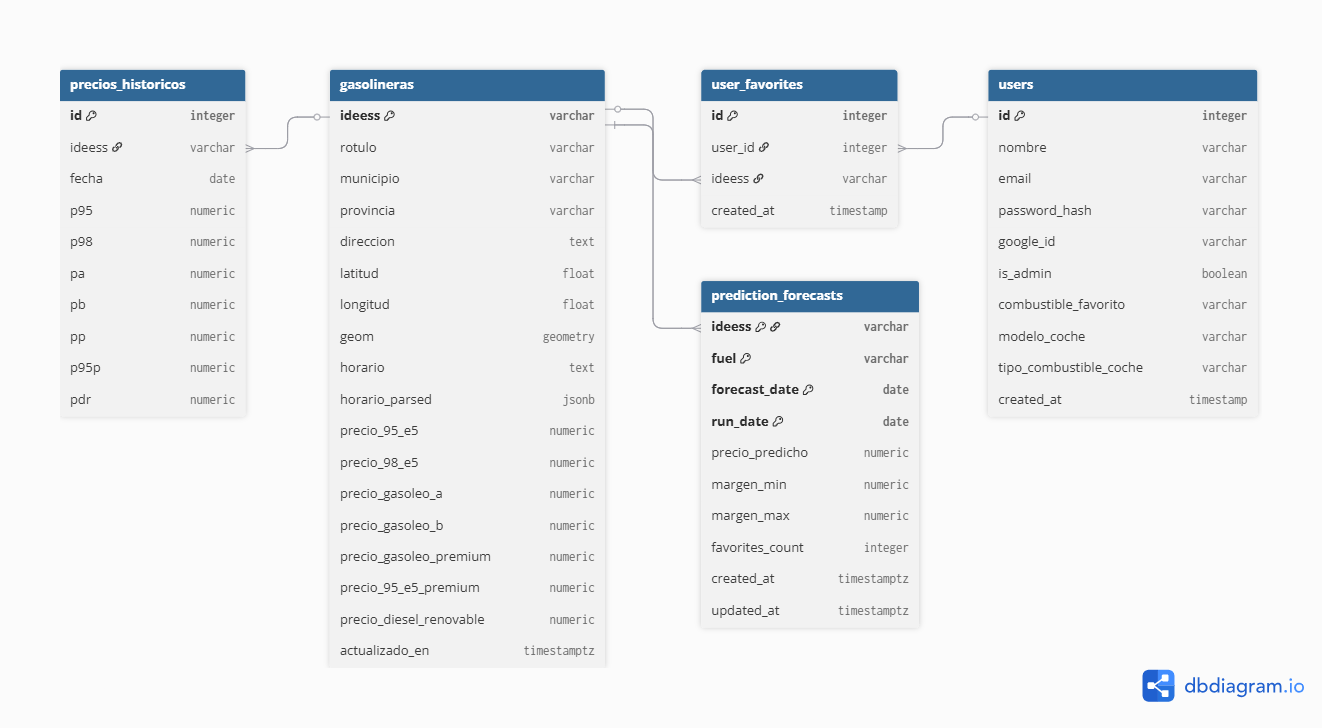
\includegraphics[width=0.85\textwidth]{imgs/entidad-relacion.png}
  \caption{Modelo entidad-relación del sistema}
  \label{fig:er}
\end{figure}

\subsection{Diagramas UML}

El diagrama de casos de uso recoge las interacciones entre los actores del sistema y sus
funcionalidades. El \textit{usuario no registrado} puede visualizar gasolineras en mapa y
tabla, consultar el mapa de electrolineras y registrarse o iniciar sesión. El
\textit{usuario registrado} extiende esas capacidades con acceso a la tabla de
electrolineras, la planificación de rutas con recomendación de repostaje, el asistente
conversacional, la predicción de precios a 7 días, la gestión de favoritos y el histórico
de precios. El sistema interactúa además con tres actores externos: la API del Ministerio
(MITECO) para la sincronización de precios, la Reve API para los puntos de recarga
eléctrica, y OpenRouteService para el cálculo de rutas.

\begin{figure}[H]
  \centering
  %\includegraphics[width=0.85\textwidth]{imgs/casos-uso.png}
  \caption{Diagrama de casos de uso del sistema}
  \label{fig:casos_uso}
\end{figure}

El diagrama de secuencia de la figura~\ref{fig:secuencia_consulta} ilustra el flujo de
consulta de gasolineras cercanas: el usuario activa la geolocalización, el frontend envía
la petición al API Gateway, este la enruta al servicio de gasolineras, que ejecuta una
consulta geoespacial sobre PostgreSQL mediante PostGIS y devuelve el listado de estaciones
con sus precios actuales para su renderizado en tabla y mapa.

\begin{figure}[H]
  \centering
  %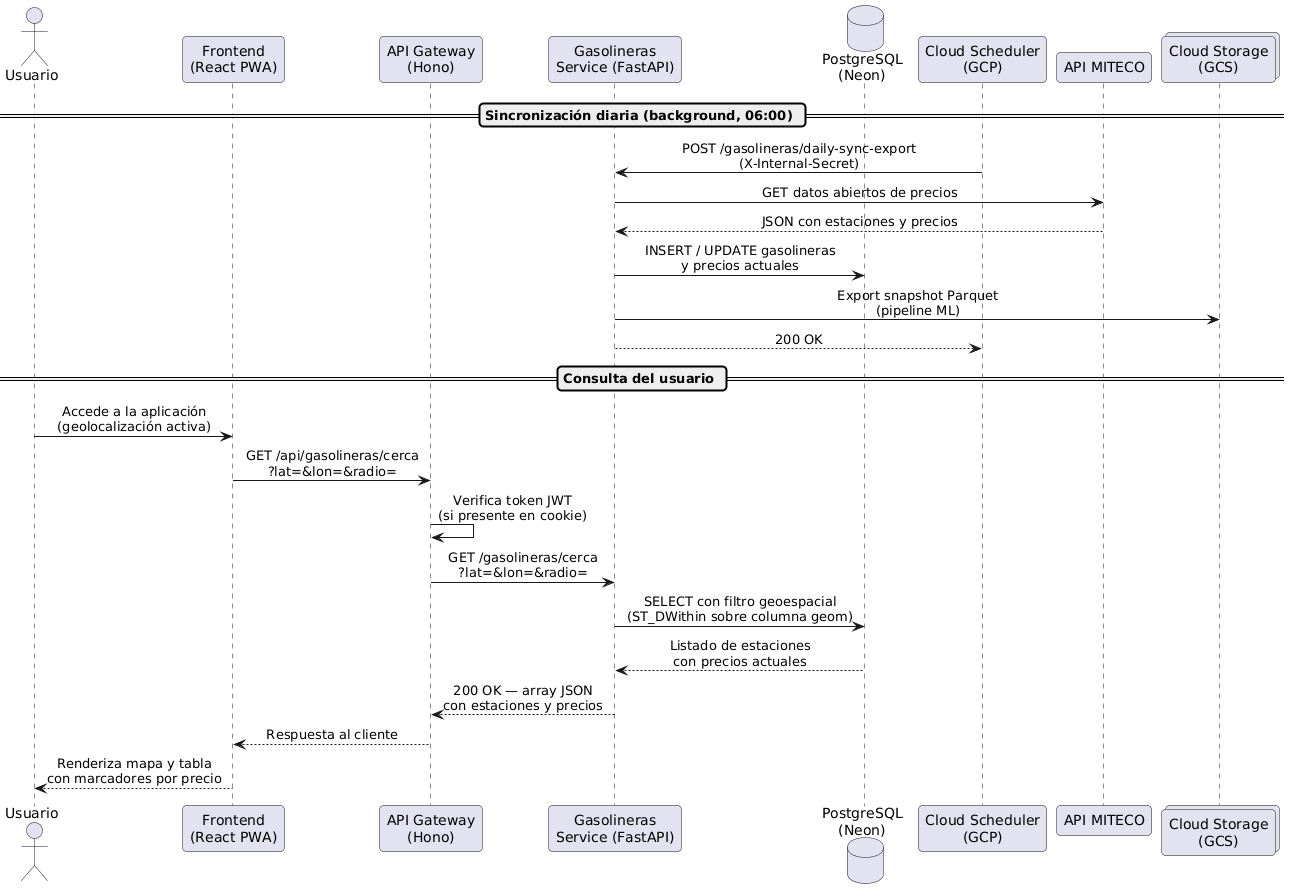
\includegraphics[width=0.85\textwidth]{imgs/secuencia-consulta.png}
  \caption{Diagrama de secuencia: consulta de gasolineras cercanas}
  \label{fig:secuencia_consulta}
\end{figure}

El segundo diagrama de secuencia, figura~\ref{fig:secuencia_ruta}, muestra el flujo de
planificación de ruta con recomendación de repostaje. El servicio de recomendación
coordina dos llamadas externas: a OpenRouteService para obtener el trazado de la ruta, y
al servicio de gasolineras para recuperar las estaciones cercanas al recorrido. Con ambas
respuestas aplica el algoritmo de ponderación por precio y desvío y devuelve las paradas
sugeridas al usuario.

\begin{figure}[H]
  \centering
  %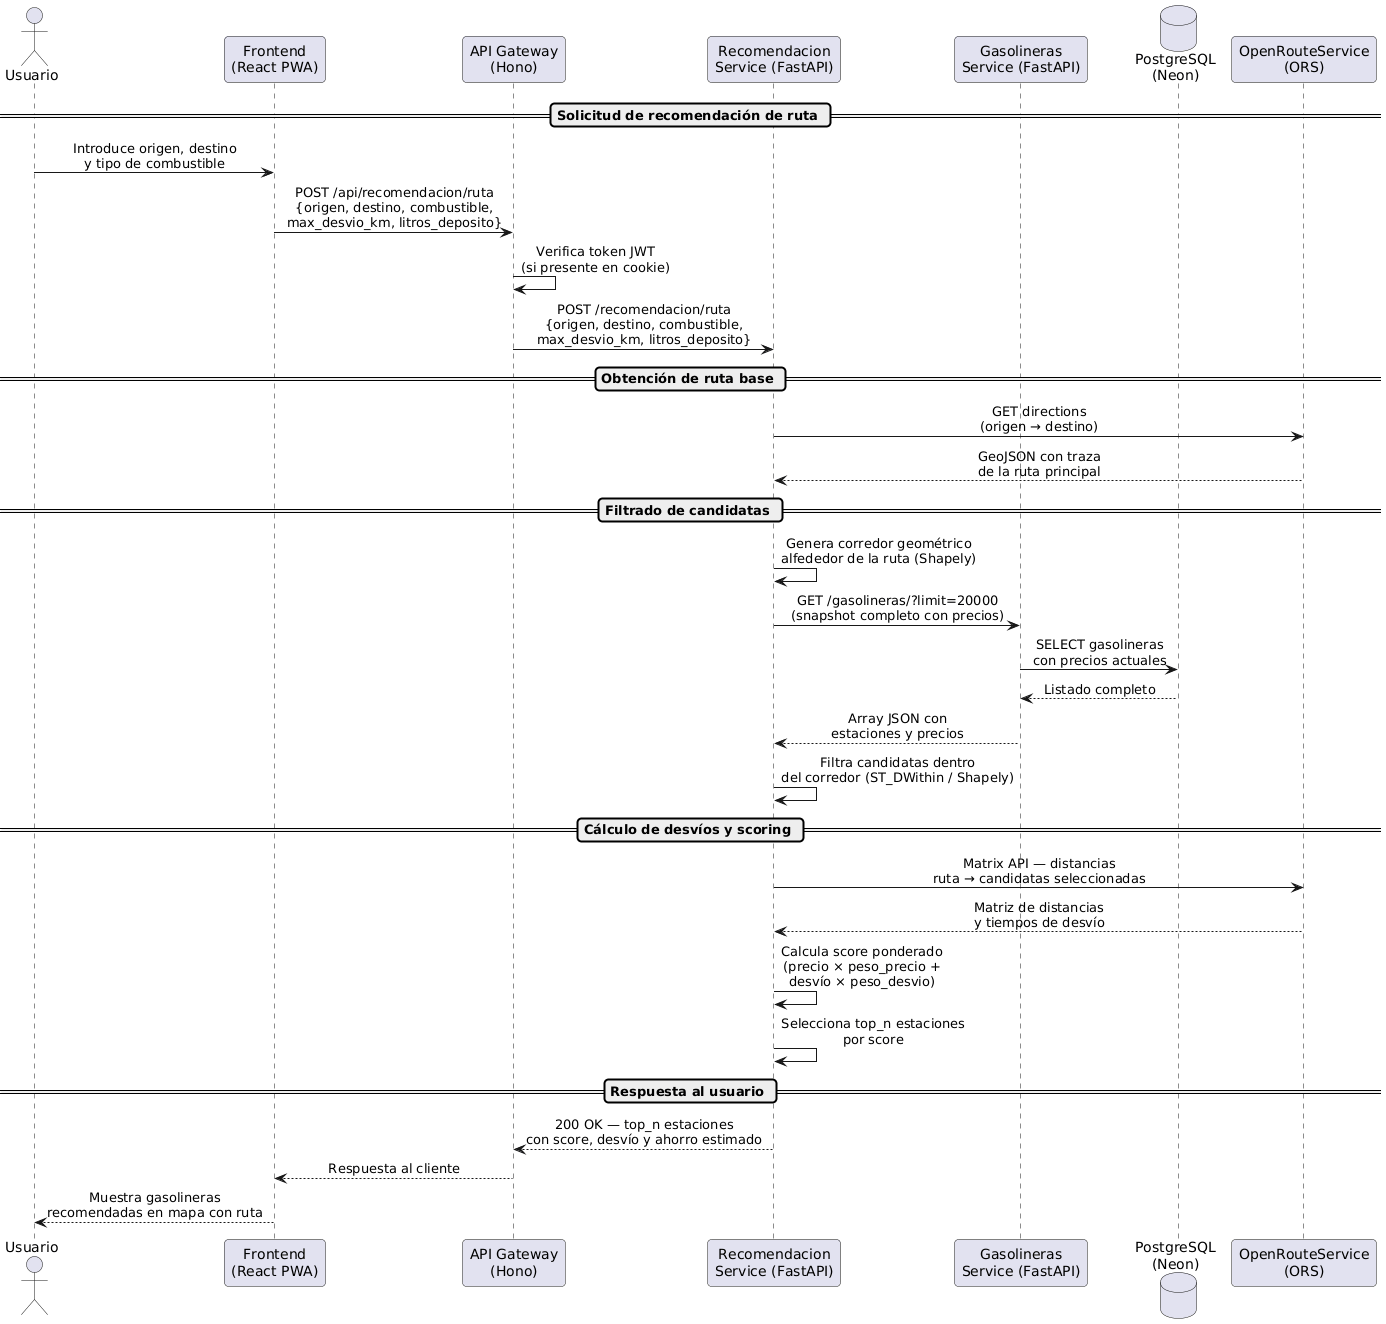
\includegraphics[width=0.85\textwidth]{imgs/secuencia-recomendacion.png}
  \caption{Diagrama de secuencia: planificación de ruta con recomendación de repostaje}
  \label{fig:secuencia_ruta}
\end{figure}

% ═════════════════════════════════════════════
\section{Consideraciones sobre la Implementación}
\label{sec:implementacion}
% ═════════════════════════════════════════════

Esta sección documenta las decisiones de implementación más relevantes de cada componente
del sistema, con especial atención a los aspectos que condicionan el comportamiento en
producción y que no quedan completamente cubiertos por la especificación de requisitos o el
diseño arquitectónico.

% ─────────────────────────────────────────────
\subsection{Estructura del proyecto}
\label{subsec:estructura}
% ─────────────────────────────────────────────

El repositorio sigue una estructura de monorepo, cada microservicio reside en su propio
directorio raíz y tiene su propio \texttt{Dockerfile}, su fichero de dependencias y su
conjunto de pruebas. Esta organización permite iterar sobre un servicio sin alterar el
resto y facilita la asignación de un pipeline de CI/CD independiente a cada componente.

Los directorios principales son \texttt{gateway-hono}, \texttt{gasolineras-service},
\texttt{usuarios-service}, \\
\texttt{recomendacion-service}, \texttt{prediction-service},
\texttt{voice-assistant-service}, \texttt{mcp-gasolineras-server} y
\texttt{frontend-client}. En la raíz se encuentran el \texttt{docker-compose.yml} para el
entorno local y los siete ficheros \texttt{cloudbuild-*.yaml} para el despliegue en
producción.

La orquestación local se basa en \textbf{Docker Compose}~\cite{docker_compose}, con
dependencias de arranque declaradas explícitamente, los servicios de dominio esperan a que
la base de datos esté accesible, el gateway espera a que los servicios de dominio superen
sus \textit{health checks}, el frontend arranca únicamente cuando el gateway está
disponible. Los servicios opcionales de IA y predicción se activan mediante perfiles Docker
(\texttt{ai}, \texttt{ml})~\cite{docker_compose_profiles}, de forma que la instalación base no requiere claves de API
externas.

% ─────────────────────────────────────────────
\subsection{Servicio de gasolineras y sincronización de datos}
\label{subsec:gasolineras_impl}
% ─────────────────────────────────────────────

El \texttt{gasolineras-service} es el componente con mayor complejidad operacional del
sistema, ya que combina la gestión de datos en tiempo real con la necesidad de mantener
frescura respecto a una fuente externa que actualiza sus precios varias veces al
día~\cite{datosgob_carburantes}.

\subsubsection*{Ciclo de sincronización}

El servicio implementa tres mecanismos de sincronización complementarios. En primer lugar,
al arrancar, si la variable \texttt{AUTO\_ENSURE\_FRESH\_ON\_STARTUP} está activa, el
servicio comprueba la antigüedad de los datos almacenados y lanza una sincronización
condicional si supera el umbral configurado. En segundo lugar, en producción un
\textbf{Cloud Scheduler} de Google Cloud Platform \cite{cloud_scheduler2026,gcp_products2026}
dispara diariamente un Cloud Run Job \cite{cloud_run2026} que invoca el endpoint interno 
\texttt{POST /gasolineras/daily-sync-export}, este endpoint
sincroniza los datos desde la API del Ministerio de Industria y, a continuación, exporta
un snapshot en formato Parquet a Google Cloud Storage \cite{cloud_storage2026} para el pipeline de machine learning.
En tercer lugar, si una petición de lectura detecta que los datos superan el umbral de
antigüedad (\texttt{AUTO\_SYNC\_ON\_READ=true}), el servicio puede desencadenar una
sincronización en segundo plano, aunque en producción esta opción se mantiene desactivada
para evitar latencia impredecible.

La combinación de estos mecanismos garantiza que los datos nunca superen 24 horas de
antigüedad en producción sin necesidad de un sistema de colas externo.

\subsubsection*{Almacenamiento y consultas geoespaciales}

Los precios actuales se almacenan en la tabla \texttt{gasolineras} junto con las
coordenadas geográficas de cada estación. Para las búsquedas por proximidad se utiliza
\textbf{PostGIS}~\cite{postgis}, la extensión geoespacial de PostgreSQL, que permite
ejecutar consultas basadas en distancia con los operadores \texttt{ST\_DWithin} y
\texttt{ST\_Distance} de forma eficiente mediante índices espaciales. Esto evita el
cálculo de la distancia haversine en capa de aplicación para el filtrado inicial,
reservándolo únicamente para el refinamiento de resultados.

El histórico de precios se registra en la tabla \texttt{precios\_historicos}, donde cada
fila representa una instantánea de los precios de una estación en una fecha concreta. Este
diseño permite construir series temporales por estación y combustible, que son la entrada
del modelo de predicción.

\subsubsection*{Fallback en memoria}

Si al arrancar el servicio no dispone de conexión a la base de datos, entra en modo
\textit{memory-fallback}: carga los datos desde la última sincronización disponible en
memoria y continúa respondiendo peticiones, aunque sin capacidad de escritura. Este modo
garantiza la resiliencia ante interrupciones transitorias de conectividad con Neon, que al
ser un servicio externo puede experimentar latencias de conexión en arranques en frío
(\textit{cold starts}) de Cloud Run.

\subsubsection*{Integración de electrolineras}

Los puntos de recarga eléctrica se obtienen de la API de Mapareve~\cite{mitma_esmovilidad}
y están integrados directamente dentro del \texttt{gasolineras-service}, bajo el prefijo
de rutas \texttt{/api/charging/}. Esta decisión evita la proliferación de microservicios
para funcionalidades que comparten el mismo patrón de acceso (consulta geoespacial, caché
corta) y reduce la complejidad operacional del despliegue.

% ─────────────────────────────────────────────
\subsection{Servicio de usuarios y autenticación}
\label{subsec:usuarios_impl}
% ─────────────────────────────────────────────

El \texttt{usuarios-service} gestiona el ciclo completo de identidad: registro,
autenticación tradicional, autenticación federada con Google OAuth y gestión de favoritos.
Está implementado con \textbf{Fastify}~\cite{fastify}, que en combinación con el plugin 
\texttt{@fastify/jwt}~\cite{fastify_jwt} proporciona la firma y verificación de tokens sin código boilerplate.

\subsubsection*{Autenticación y tokens JWT}

Tras un inicio de sesión correcto, el servicio genera un token \textbf{JWT}~\cite{jwt_rfc}
firmado con el algoritmo HS256 y una caducidad de 7 días. El token no se devuelve en el
cuerpo de la respuesta, sino que el API Gateway lo establece como una \textit{cookie}
\texttt{httpOnly} con los flags \texttt{Secure} y \texttt{SameSite=None} en producción.
Este mecanismo impide que el token sea accesible desde JavaScript del navegador, mitigando
ataques XSS~\cite{owasp_xss}.

Para el flujo de Google OAuth, el gateway actúa como intermediario: recibe el
\texttt{id\_token} de Google, lo verifica y llama al endpoint interno
\texttt{POST /api/usuarios/google/internal} con cabecera \texttt{X-Internal-Secret}, de
forma que este endpoint nunca queda expuesto al exterior. El servicio realiza un
\textit{upsert} del usuario (crea la cuenta si no existe, o la actualiza si ya existe por
email) y devuelve el JWT al gateway para su encapsulación en cookie.

Las contraseñas se almacenan únicamente como hash generado con \textbf{bcrypt}~\cite{bcrypt}
con 12 rondas de sal, lo que hace computacionalmente inviable su recuperación por fuerza
bruta incluso en caso de exfiltración de la base de datos.

\subsubsection*{Gestión del esquema de base de datos}

El proyecto no utiliza un sistema de migraciones automático tipo Flyway o Liquibase. El
esquema se define en un fichero \texttt{init.sql} con sentencias idempotentes
(\texttt{CREATE TABLE IF NOT EXISTS}, \texttt{ALTER TABLE IF NOT EXISTS}) que se aplican
manualmente sobre la instancia PostgreSQL de Neon en el primer despliegue. Esta decisión
es apropiada para el alcance del proyecto, aunque en un sistema de producción con múltiples
entornos sería recomendable introducir un gestor de migraciones formal para controlar la
evolución del esquema a lo largo del tiempo.

\subsubsection*{Rate limiting}

Los endpoints de registro e inicio de sesión aplican un límite de 5 peticiones por IP
cada 15 minutos mediante el plugin \texttt{@fastify/rate-limit}~\cite{fastify_ratelimit},
configurado con \texttt{global: false} para no afectar al resto de rutas. Las direcciones
de loopback (\texttt{127.0.0.1}, \texttt{::1}) quedan exentas para no interferir con las
pruebas locales.

% ─────────────────────────────────────────────
\subsection{Servicio de recomendación de ruta}
\label{subsec:recomendacion_impl}
% ─────────────────────────────────────────────

% Pendiente de desarrollar — el servicio de recomendación aún está en fase de refinamiento.

% ─────────────────────────────────────────────
\subsection{Módulo de predicción de precios}
\label{subsec:prediccion_impl}
% ─────────────────────────────────────────────

El \texttt{prediction-service} implementa un pipeline de machine learning para estimar el
precio de combustible de las estaciones favoritas de los usuarios durante los próximos 7
días. El diseño se orienta a la ejecución periódica en lote (\textit{batch}) más que a la
inferencia en tiempo real.

\subsubsection*{Selección del modelo}

Se evaluaron varios enfoques de regresión para series temporales: modelos ARIMA clásicos,
redes LSTM y árboles potenciados por gradiente. Se ha optado por \textbf{LightGBM}~\cite{lgbm}
en régimen de \textbf{regresión cuantílica} por tres razones principales. Primero, ofrece
un rendimiento muy competitivo en tablas de series temporales con features derivadas sin
requerir la normalización y el ajuste de hiperparámetros extensivo que exigen las redes
neuronales recurrentes. Segundo, la regresión cuantílica (cuantiles 0.05, 0.50, 0.95)
produce directamente intervalos de confianza para cada predicción, lo que enriquece la
información presentada al usuario. Tercero, LightGBM tiene un tiempo de entrenamiento muy
reducido, compatible con la ejecución semanal del job en un entorno serverless con límites
de memoria y CPU~\cite{ke2017lightgbm}.

\begin{figure}[H]
  \centering
  %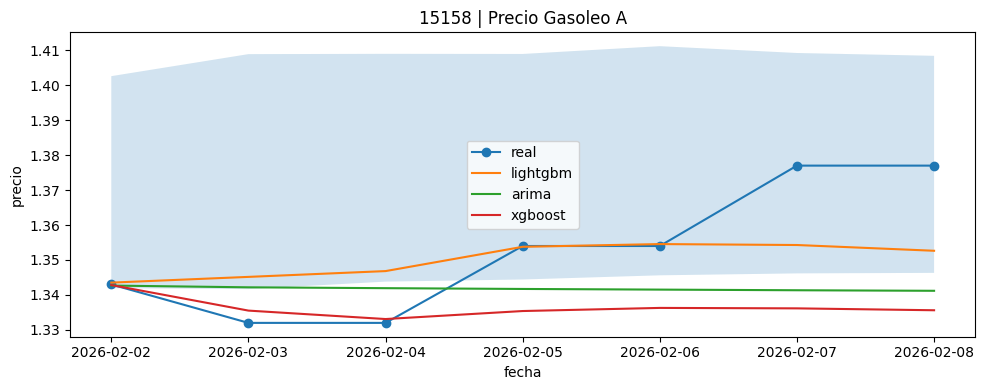
\includegraphics[width=0.85\textwidth]{imgs/prediccion_mae_comparativa.png}
  \caption{Comparativa de MAE entre modelos evaluados durante el desarrollo}
  \label{fig:mae_comparativa}
\end{figure}

\subsubsection*{Ingeniería de \textit{features}}

Para cada estación y tipo de combustible se construye una serie temporal diaria con el
precio medio registrado. A partir de ella se generan \textit{features} temporales
(día de la semana, fin de semana, semana del año, mes, trimestre), \textit{lags} de 1, 7,
14, 21 y 30 días, medias móviles y desviaciones típicas de ventanas de 7, 14 y 30 días,
y diferencias a 1 y 7 días. Adicionalmente, si la conexión a internet está disponible,
se descarga el precio del crudo Brent mediante \textbf{yfinance}~\cite{yfinance} y se
incorporan sus lags como variable exógena, aprovechando la correlación conocida entre el
precio del petróleo y los precios en surtidor~\cite{LAHMIRI2024105008}.

\subsubsection*{Ciclo de entrenamiento e inferencia}

El pipeline se ejecuta semanalmente mediante un \textbf{Cloud Run Job} disparado por
\textbf{Cloud Scheduler} (cada lunes a las 06:00 UTC). En cada ejecución, el job descarga
los snapshots Parquet de los últimos 180 días desde Google Cloud Storage, valida que los
datos estén frescos, reentrena el modelo para cada par (estación, combustible), genera
las predicciones de los 7 días siguientes de forma secuencial —cada día nuevo utiliza las
predicciones previas para recalcular los lags— y persiste los resultados en la tabla
\texttt{prediction\_forecasts} de PostgreSQL. Los artefactos del modelo entrenado
(\texttt{.pkl}) se almacenan en el bucket GCS bajo el prefijo \texttt{modelos\_lgbm/}
para su eventual reutilización.

La selección de estaciones a predecir se basa en los favoritos globales de los usuarios:
el job consulta el endpoint interno \texttt{/api/usuarios/favoritos/all-ideess} para
obtener los identificadores únicos de las estaciones con al menos un usuario que las ha
marcado como favoritas. Este criterio concentra la capacidad de cómputo en las estaciones
con mayor demanda real, evitando el coste prohibitivo de entrenar modelos para las más
de 11\,000 estaciones del catálogo nacional.

\subsubsection*{Consulta de predicciones}

En producción el servicio opera en modo API (\texttt{RUN\_HTTP\_API=true}): no ejecuta el
pipeline de entrenamiento, sino que expone el endpoint
\texttt{GET /api/prediction/station/\{ideess\}} que lee directamente de la tabla
\texttt{prediction\_forecasts}. El entrenamiento y la escritura en base de datos son
responsabilidad exclusiva del Cloud Run Job periódico, separando claramente los roles de
escritura y lectura.

% ─────────────────────────────────────────────
\subsection{Asistente conversacional de voz}
\label{subsec:voice_impl}
% ─────────────────────────────────────────────

El \texttt{voice-assistant-service} implementa un asistente de dominio restringido que
permite al usuario realizar consultas sobre gasolineras en lenguaje natural, tanto por
texto como por voz, y recibir una respuesta en audio. El servicio está implementado con
\textbf{Fastify}~\cite{fastify} y se integra con la API de \textbf{Google Gemini}~\cite{gemini}
mediante llamadas HTTP REST al cliente \texttt{@google/genai}.

\subsubsection*{Pipeline STT $\rightarrow$ LLM $\rightarrow$ TTS}

El pipeline se ejecuta en tres etapas secuenciales, cada una con su propia llamada a la
API de Gemini. En la etapa de \textbf{reconocimiento de voz} (\textit{Speech-to-Text}),
si la petición incluye audio en base64, el servicio invoca \texttt{generateContent} con
el modelo configurado para transcribir el audio a texto. En la etapa de \textbf{razonamiento}
(\textit{LLM con function calling}), se realiza una primera llamada con las declaraciones
de las funciones disponibles (\texttt{get\_prices} y \texttt{get\_nearest\_stations}); si
el modelo solicita ejecutar alguna de ellas, el servicio las invoca localmente contra el
API Gateway y realiza una segunda llamada con los resultados, obteniendo así la respuesta
final fundamentada en datos reales. En la etapa de \textbf{síntesis de voz}
(\textit{Text-to-Speech}), se realiza una llamada adicional a Gemini con modalidad de
respuesta \texttt{AUDIO}, la respuesta PCM se convierte a WAV y se devuelve en base64
al cliente.

Este diseño con tres llamadas separadas, en lugar de una única llamada multimodal, ofrece
mayor control sobre cada etapa y facilita el manejo de errores y los fallbacks por modelo.

\subsubsection*{Guardarraíles y control del dominio}

Dado que el asistente está diseñado para un dominio muy específico, se implementan varios
mecanismos para evitar un uso fuera de ámbito. Un \textbf{comprobador de alcance}
(\textit{scope guard}) basado en palabras clave evalúa la transcripción antes de invocar
el LLM; si la consulta no contiene términos relacionados con combustible, gasolineras,
precios o navegación, y la variable \texttt{VOICE\_GUARDRAILS\_ENABLED} está activa, el
servicio devuelve una respuesta predefinida sin consumir tokens del modelo. El modo
\texttt{strict} rechaza directamente la petición; el modo \texttt{soft} permite continuar
con una advertencia al modelo.

Adicionalmente, el \textbf{system prompt} construido por \texttt{buildSystemInstruction}
instruye explícitamente al modelo sobre el idioma, el tono y el formato esperados, y lo
obliga a utilizar las funciones declaradas para cualquier consulta de datos, reduciendo el
riesgo de alucinaciones. El function calling se ejecuta en el servidor, de forma que el
LLM nunca interactúa directamente con el gateway, sino que proporciona los parámetros de
la llamada y espera los resultados.

Otros controles operativos incluyen límites de tamaño de payload
(\texttt{VOICE\_MAX\_TEXT\_CHARS}, \texttt{VOICE\_MAX\_AUDIO\_BASE64\_CHARS}), timeouts
por llamada a Gemini con \texttt{AbortController}, y rate limiting por IP para el
transporte WebSocket. Como limitación conocida, el rate limiter no se aplica actualmente
al endpoint HTTP \texttt{/voice/dialog}, aspecto identificado para una iteración futura.

\subsubsection*{Nota sobre el transporte WebSocket}

El servicio implementa tanto el endpoint HTTP \texttt{POST /voice/dialog} como un
endpoint WebSocket \texttt{/ws/voice} para streaming de audio. Durante el desarrollo se
identificaron problemas de estabilidad de conexión con el transporte WebSocket en el
entorno de Cloud Run, asociados al comportamiento de las peticiones de larga duración en
infraestructura serverless. Por ello, el cliente frontend utiliza actualmente el endpoint
HTTP, que ofrece un comportamiento predecible en todos los entornos de despliegue.

% ─────────────────────────────────────────────
\subsection{Frontend: React PWA con Nginx}
\label{subsec:frontend_impl}
% ─────────────────────────────────────────────

El frontend es una \textit{Single Page Application} (SPA) construida con
\textbf{React 19}~\cite{react} y \textbf{TypeScript}~\cite{typescript}, compilada con
\textbf{Vite}~\cite{vite} y empaquetada como \textbf{Progressive Web App}
(PWA)~\cite{pwa_spec}. En producción, los artefactos estáticos generados por Vite se
sirven mediante \textbf{Nginx}~\cite{nginx} dentro de un contenedor Docker de imagen
mínima.

\subsubsection*{Configuración de Nginx}

Nginx está configurado para servir el directorio \texttt{dist} generado por Vite desde
\texttt{/usr/share/nginx/html}. La directiva \texttt{try\_files \$uri \$uri/ /index.html}
garantiza que todas las rutas no estáticas sean resueltas por el router de React en
cliente, comportamiento necesario para el correcto funcionamiento de la navegación SPA.
Los assets estáticos con huella de contenido (\texttt{.js}, \texttt{.css}, fuentes e
imágenes) se cachean durante un año con la cabecera
\texttt{Cache-Control: public, immutable}, lo que maximiza el rendimiento en visitas
recurrentes. Nginx no actúa como proxy inverso para la API en producción: todas las
llamadas al backend se dirigen directamente a la URL del API Gateway configurada en
tiempo de compilación mediante la variable \texttt{VITE\_API\_BASE\_URL}.

\subsubsection*{Progressive Web App}

La aplicación implementa el estándar PWA mediante el plugin
\textbf{vite-plugin-pwa}~\cite{vite_pwa} con Workbox~\cite{workbox} como gestor del
Service Worker. El fichero \texttt{manifest.webmanifest} define los metadatos necesarios
para la instalación en dispositivos móviles (nombre, iconos, color de tema y modo de
visualización \textit{standalone}). El Service Worker implementa una estrategia de caché
que permite el acceso a la interfaz aunque la conexión sea intermitente, aunque las
consultas de datos en tiempo real requieren conectividad activa.

\subsubsection*{Internacionalización y diseño responsivo}

La interfaz soporta tres idiomas (español, inglés y euskera) mediante
\textbf{i18next}~\cite{i18next} con detección automática del idioma del navegador. El
diseño sigue un enfoque \textit{mobile-first} con \textbf{TailwindCSS}~\cite{tailwind},
garantizando que la experiencia sea funcional tanto en pantallas de escritorio como en
dispositivos móviles, donde el caso de uso de búsqueda de gasolineras en ruta es
predominante. El mapa interactivo se implementa con \textbf{Leaflet}~\cite{leaflet} a
través de la librería \texttt{react-leaflet}, con soporte para clustering de marcadores
a niveles de zoom bajos para evitar la saturación visual cuando hay muchas estaciones en
el área visible.

% ─────────────────────────────────────────────
\subsection{Despliegue en GCP y pipeline CI/CD}
\label{subsec:despliegue_impl}
% ─────────────────────────────────────────────

Todos los microservicios se despliegan en \textbf{Google Cloud Run}~\cite{cloud_run},
plataforma serverless que gestiona el escalado automático en función de la demanda y
factura únicamente por el tiempo de cómputo efectivo. Esta elección elimina la necesidad
de gestionar instancias o clústeres, lo que reduce significativamente la carga operacional
para un proyecto académico sin comprometer la disponibilidad.

\subsubsection*{Pipeline de CI/CD}

Cada microservicio dispone de su propio fichero \texttt{cloudbuild-*.yaml} que define un
pipeline de \textbf{Cloud Build}~\cite{cloud_build} independiente. Los pipelines se
activan automáticamente con cada \textit{push} a la rama \texttt{main} del repositorio.
El proceso consta de tres pasos: construcción de la imagen Docker, publicación en
\textbf{Artifact Registry}~\cite{artifact_registry} (región \texttt{europe-west1}), y
despliegue en Cloud Run con las variables de entorno inyectadas desde
\textbf{Secret Manager}~\cite{secret_manager}. Este diseño garantiza que ningún secreto
esté presente en el repositorio ni en los logs de compilación.

El pipeline del frontend incluye validaciones adicionales en el paso de compilación: la
variable \texttt{VITE\_API\_BASE\_URL} debe apuntar a un dominio HTTPS (no a
\texttt{localhost}), lo que previene despliegues accidentales de configuraciones de
desarrollo.

\subsubsection*{Comunicación entre servicios en Cloud Run}

En Cloud Run cada servicio tiene una URL pública asignada por Google, pero la comunicación
interna entre servicios no debe transitar por internet. Para ello, el gateway utiliza
tokens IAM de servicio (\textit{service account tokens}) inyectados mediante el módulo
\texttt{cloudRunAuthFetch.js}, que autentica cada llamada inter-servicio ante la
infraestructura de Google sin exponer los servicios internos a peticiones externas no
autorizadas.

\subsubsection*{Base de datos y almacenamiento}

La base de datos PostgreSQL reside en \textbf{Neon Tech}~\cite{neon}, proveedor de
PostgreSQL serverless que ofrece \textit{branching} de bases de datos, hibernación
automática de instancias inactivas y conexión mediante cadena estándar
\texttt{postgresql://}. La elección de un proveedor externo en lugar de Cloud SQL de GCP
responde a la disponibilidad de un plan gratuito suficiente para las cargas del proyecto
y a la independencia del proveedor cloud para la capa de datos.

Los snapshots Parquet del pipeline de ML y los modelos entrenados se almacenan en
\textbf{Google Cloud Storage}~\cite{gcs}, que actúa como capa de almacenamiento de objetos
entre el servicio de gasolineras (productor de datos), el job de predicción (consumidor y
productor de modelos) y el servicio de predicción en modo API (lector de resultados).

% ─────────────────────────────────────────────
\subsection{Seguridad transversal}
\label{subsec:seguridad_impl}
% ─────────────────────────────────────────────

Además de los mecanismos de autenticación descritos en la sección anterior, el sistema
implementa un conjunto de controles de seguridad aplicados de forma transversal.

La comunicación entre el gateway y los microservicios internos está protegida por la
cabecera \texttt{X-Internal-Secret}: los endpoints de administración (sincronización
forzada, export, consulta de favoritos globales) rechazan con \texttt{403 Forbidden}
cualquier petición que no incluya el secreto configurado en \texttt{INTERNAL\_API\_SECRET}.
Este mecanismo evita que dichos endpoints sean accesibles desde el exterior incluso si
un servicio queda expuesto inadvertidamente.

La validación de datos de entrada se realiza en capa de aplicación con
\textbf{Pydantic v2}~\cite{pydantic} en los servicios Python y con los esquemas de
validación de Fastify en los servicios Node.js. Los parámetros de consulta con potencial
de abuso (radio de búsqueda, límite de resultados) tienen cotas máximas declaradas
explícitamente. Las consultas a PostgreSQL utilizan siempre parámetros preparados, sin
concatenación de cadenas, eliminando el vector de inyección SQL~\cite{owasp_sqli}.

El servicio de usuarios aplica \textbf{Helmet.js}~\cite{helmetjs} para establecer
cabeceras HTTP de seguridad (\texttt{X-Frame-Options}, \texttt{Content-Security-Policy},
\texttt{X-Content-Type-Options}). En producción, Cloud Run gestiona HTTPS
automáticamente, de forma que todo el tráfico externo está cifrado en tránsito. Los
secretos de producción (claves de API, cadenas de conexión, JWT secret) nunca residen en
el repositorio y se inyectan en tiempo de ejecución desde Secret Manager.
\section{Plan de Pruebas}
\subsection{Estrategia}
\subsection{Pruebas unitarias}
\subsection{Pruebas de integración}
\subsection{Pruebas funcionales}
\subsection{Resultados obtenidos}

\section{Manual de Usuario}
\subsection{Acceso al sistema}
\subsection{Uso de la plataforma}
\subsection{Capturas de pantalla}

\section{Incidencias del Proyecto}




%% ----------------------
%% Bibliografía y apéndices
%% ----------------------

\backmatter

\bibliografia{referencias}  % Archivo BibTeX: referencias.bib

\appendix
\chapter{Ejemplo Apéndice 1}

\end{document}
